\documentclass[12pt,a4paper]{report}
\usepackage{bm}
\usepackage[T1]{fontenc}
\usepackage[utf8]{inputenc}
\usepackage[english]{babel}
\usepackage{lmodern}
%\usepackage{circuitikz}
\usepackage{color}
\usepackage{wrapfig}
\usepackage{placeins}
\usepackage{subfigure}
\usepackage{tabu}
%\usepackage{fullpage}
\usepackage[squaren]{SIunits}
\usepackage{graphicx}
%\usepackage[pdftex]{graphicx}
\usepackage{epstopdf}
\usepackage{epsfig}
\usepackage{hyperref}
\usepackage{tikz}
\usepackage{tikz-qtree}
\usepackage{eurosym}
%\usepackage{chemist}
\usepackage{amsmath}
\usepackage{amssymb}
\usepackage{amsthm}
\usepackage{mathrsfs}
\usepackage{commath}
\usepackage{dsfont}
\usepackage{tikz}
\usetikzlibrary{arrows,automata}
\usepackage{pgfplots}
\usepackage{graphicx}
\usepackage{setspace}
\usepackage{listings}
\usepackage{amsmath}
\usepackage{algorithm}
\usepackage[noend]{algpseudocode}
%\usepackage[section]{placeins}
\usepackage{pdflscape}
\usepackage{MnSymbol}

\usepackage{natbib}
\usepackage{graphicx}
\usepackage{enumitem}
\title{Thesis}
\author{Garrett Thomas}

%\theoremstyle{definition}
\newtheorem{definition}{Definition} % definition numbers are dependent on theorem numbers
\newtheorem{theorem}{Theorem} % same for example numbers
\newtheorem{assumption}{Assumption} % same for example numbers
\newtheorem{problem}{Problem} % same for example numbers
\newtheorem{remark}{Remark}
\newtheorem{lemma}{Lemma}
\newtheorem{corollary}{Corollary}
\newtheorem{example}{Example}

\makeatletter
\def\BState{\State\hskip-\ALG@thistlm}
\makeatother

\floatname{algorithm}{Procedure}
\renewcommand{\algorithmicrequire}{\textbf{Input:}}
\renewcommand{\algorithmicensure}{\textbf{Output:}}

\newcommand{\R}{\mathbb{R}}
\newcommand{\F}{\mathcal{F}}
\newcommand{\Q}{\mathcal{Q}}
\newcommand{\T}{\mathcal{T}}
\newcommand{\A}{\mathcal{A}}
\newcommand{\Inf}{\texttt{Inf}}
\newcommand{\Post}{\texttt{Post}}
\newcommand{\Pre}{\texttt{Pre}}
\newcommand{\Edge}{\texttt{Edge}}
\newcommand{\Cost}{\texttt{Cost}}
\newcommand{\trace}{\texttt{trace}}
\newcommand{\U}{\bm{\mathcal{U}}}
\newcommand{\ssquare}{\text{\scalebox{0.6}{$\square$}}}
%$\square$ {\scriptsize $\square$} $\circ$ \scalebox{0.6}{$\square$}

\usepackage{makecell}

\renewcommand\theadalign{cb}
\renewcommand\theadfont{\bfseries}
\renewcommand\theadgape{\Gape[4pt]}
\renewcommand\cellgape{\Gape[4pt]}

\lstset{breaklines=true}
\begin{document}

\maketitle
\tableofcontents
\newpage
\listoffigures
\newpage
\FloatBarrier
\chapter{Introduction}
\section{Problem}
The use of formal methods, specifically \textit{model checking}, in control planning synthesis is a new and exciting research area. Formal methods are originally mathematical techniques to specifiy and verify the design of software and hardware \cite{clarke96}. \textit{formal verification} methods ensure that there are no bugs present in the software or hardware design which will cause unexpected behaviors. This is needed because other debugging techniques such as simulation and testing only ensure that there are no problems with a given the input. Bugs that go undetected can have disastrous effects, such as the explosion of the Ariane 5 rocket in 1996, which was caused by an exception being thrown when a 64-bit floating point number was converted to a 16-bit signed integer \cite{clarke99}. 

%This is however not what model checking was originally designed for. Model checking was designed as a method for . When designing software or hardware one wants to make sure that it does what it is supposed to do, and that there are no bugs in the program which will cause unexpected behaviors. These bugs can have disastrous effects, such as the explosion of the Ariane 5 rocket in 1996, which was caused by an exception being thrown when a 64-bit floating point number was converted to a 16-bit signed integer \cite{clarke99}. 
Model checking is an approach to formal verification which decides if a model of the program satisfies some behavior. These behaviors can be given as a temporal logic formula, commonly linear temporal logic (LTL) or computation tree logic (CTL). Since its advent, model checking under temporal logics has proved to be a very useful tool in software and hardware development. There are commercial and open source model checkers available \cite{holzmann03}, \cite{cimatti02} and many companies have their own in house model checking programs. 

Two main benefits of model checking are that 1) it is completely autonomous; after the program is modelled and the behavior is formalized into temporal logic, the model checker is self sufficient and no longer requires user interaction and 2) in the situation when the model fails to satisfy the given formula, a counter example is given (\textit{why} the model does not satisfy the specification). 

%The latter property gives valuable information for debugging purposes, and also 
It is obvious to see how the counter example gives valuable information for debugging purposes. This counter example however has also given rise to the new and exciting field of model planning as a tool for control planning synthesis. In this field of motion and task planning, the model of the program is replaced by a model of the robot's environment and the formula is the \textit{negation} of the desired robot motion and tasks. The realization that the double negative of a \textit{counter example} of the \textit{negation} of the desired motion was in fact the desired motion is the basis of this field. Earlier works in this field have even used the same programs that were designed for classic model checking \cite{fainekos05}. %spin is used in blah blah blah papers

Model checking however is not perfect. It suffers from what is known as the \textit{state-space explosion problem}. This is a phenomenon in which the number of states can quickly grow to an unmanageable number rendering the model checking uncomputable. Neither classical model checking or the application of model checking in motion planning is safe from the state explosion problem, however techniques have been developed to address this problem in classical model checking. These techniques include partial order reduction and abstraction, among others. Partial order reduction consists of trying to reduce the number of independent interleavings of concurrent processes, while abstraction attempts to simplify the model. These techniques have proved useful for classical model checking, however they unfortunately have limited applicability in model checking for robot motion.  
% e.g. ignore non-boolean variables in the model !!give citation!!

To address the state space explosion problem, we are presenting a method that does not reduce the number of states. It does however speed up the following search through the states. Instead of an algorithm that computes the globally optimal path, we instead propose an algorithm that takes the optimal path at each step according to the greedy paradigm. The performance of our proposed algorithm is then analysed in the context of robot motion planning and compared to the accepted algorithm from the literature. The algorithm is also applicable to classical model checking, however this is out of the scope of this work. 

\section{Outline}
\begin{description}
    \item[Chapter 2] We will first present all the theoretical results necessary for understanding the technique of model checking for motion planning. This will be self contained and does not require any prior knowledge in the field.
    \item[Chapter 3] We will review the current algorithm that is accepted and widely used and also our algorithm. We will review key differences in the procedures.
    \item[Chapter 4] We will test both algorithms on various formulas common in the field of motion planning for robot motion. The results are compared. %MAke a distinction between motion planning and task planning!! and stick to it!!!
    \item[Chapter 5] We will move on to more complex formulas including mixtures of motion planning and task planning. The results of the two algorithms are compared. 
    \item[Chapter 6] We draw conclusions and give recommendations of possible future work.
\end{description}

%which can be used for model checking, however we choose to only focus on LTL formulas. 
\newpage
\FloatBarrier
\chapter{Theoretical Background}
In this chapter we provide the theoretical background that is needed to understand control planning synthesis and linear temporal logic. 
\section{Abstraction of the Workspace}
In \cite{belta07}, Belta et al describe robot path planning as consisting of three parts: the specification level, execution level, and the implementation level. The first level, the specification level, involves creating a graph that represents the robot motion. Next is the execution level, which involves finding a path through the graph that satisfies a specification. Lastly, in the implementation level controllers are constructed that satisfy the path found in the previous step. 

We assume that we have one robot which is located in a given workspace denote $W_0 \subset \mathbb{R}^n$, which is bounded. To represent our workspace (which is a subspace of $\mathbb{R}^n$) in a finite graph we must partition it into a finite number of equivalence classes. A partition map is formally defined in definition \ref{def:PM}. Any partition can be used as long as it satisfies the bisimulation property \cite{belta04}, which will be defined later once more notation has been introduced. We denote the $\Pi = {\pi_1, \pi_2, \dots, \pi_w}$ to be the set of equivalence classes the workspace has been partitioned into, and thus $\cup_{i=1}^w \pi_i = W_0$ and $\pi_i \cap \pi_j = \emptyset$, $\forall i,j=1,2,\dots,w$ and $i\neq j$. We will henceforth refer to equivalence class $\pi_i$ as region $\pi_i$ for $i = 0,1,\dots, w$. 

\begin{definition}
\label{def:PM}
A partition map, $T: W_0 \rightarrow \Pi$ sends each state $x \in W_0$ to the finite set of equivalence classes $\Pi = {\pi_i}$,  $i = 1,2,\dots ,w$. $T^{-1}(\pi_i)$ is then all the states $x \in W_0$ that are in the equivalence class $\pi_i$ \cite{fainekos05}. 
\end{definition} 

We now introduce atomic propositions, which will be the building blocks for our task specification. Atomic propositions are boolean variables, and will be used to express properties about the state, the robot or the workspace. We define the following set of atomic propositions $AP_r = \{\alpha_{r,i}\}$, $i=1,2,\dots,w$ where 
\[\alpha_{r,i} =  \begin{cases}
\top & \text{if the robot is in region $\pi_i$} \\
\bot & \text{else}
\end{cases}
\]
which represent the robot's location \cite{guo15}. Other things we want to be able to express are potential tasks, denote $AP_p = \{\alpha_{p,i}\}$, $i=1,2,\dots,m$. These can be statements such as "there is a ball in region $\pi_I$" or "the robot beeps"
We now define the set of all propositions $AP = AP_r \cup AP_p$.

\theoremstyle{definition}
\begin{definition}
\label{defCLF}
The continuous labelling function $L_C:W_0 \rightarrow 2^{AP}$ maps a point $x \in W_0$ to the set of atomic propositions satisfied by $x$ \cite{guo15}.
\end{definition} 

We also include a definition of the discrete counterpart 

\theoremstyle{definition}
\begin{definition}
\label{defDLF}
The labelling function $L_D:\Pi\rightarrow 2^{AP}$ maps a region $\pi_i \in \Pi$ to the set of atomic propositions satisfied by $\pi_i$.
\end{definition} 
Note: $2^{AP}$ is the powerset of $AP$, i.e.\ the set of all subsets of $AP$ include the null set and $AP$. For example, by definition, $\alpha_{r,i} \in L_D(\pi_i)$. 

To define a graph that represents our environment, we must also consider the dynamics of the robot. The dynamics are relevant because they define the relationship between the various regions. The relationship we refer to is known as a transition. We define a transition between two points in $W_0$ as follows
\theoremstyle{definition}
\begin{definition}
\label{defCTransition}
There is a continuous transition, $\rightarrow_C \subset W_0 \times W_0$ from $x$ to $x'$, denoted $x \rightarrow_C x'$ if it is possible to construct a trajectory $x(t)$ for $0 \leq t \leq T$ with $x(0)=x$ and $x(T) =x'$ and we have $x(t) \in (T^{-1}(T(x))\cup T^{-1}(T(x')))$ \cite{fainekos09}
\end{definition}

We then say that there is a transition between two regions if from any point in the first region there is a transition to a point in the second region. More formally

\theoremstyle{definition}
\begin{definition}
\label{defDTransition}
There is a discrete transition, $\rightarrow_D \subset \Pi \times \Pi$, from $\pi_i$ to $\pi_j$, denoted $\pi_i \rightarrow_D \pi_j$ if for every $x$ in $\pi_i$ i.e.\ $T(x) = \pi_i$ there exists $x'$ such that $T(x')=\pi_j$ and $x \rightarrow_C x'$
\end{definition}

We can now define bisimulations
\theoremstyle{definition}
\begin{definition}
\label{def:bisim}
A partition $T:W_0\rightarrow \Pi$ is called a bisimulation \cite{fainekos09} if the following properties hold for all $x,y \in W_0$
\begin{enumerate}
    \item (Observation Preserving): If $T(x)=T(y)$, then $L_C(x) = L_C(y)$.
    \item (Reachability Preserving): If $T(x) = T(y)$, then if $x\rightarrow_C x'$ then $y \rightarrow_C y'$ for some $y'$ with $T(x')=T(y')$
\end{enumerate}
\end{definition}

The Observation Preserving requirement makes sure we do not allow the situation where part of $\pi_i$ fulfils $\alpha \in AP$ while part of $\pi_i$ does not, and the Reachability Preserving requirement ensures that for every point in region $\pi_i$, there exists a trajectory to some point $x'$, such that $T(x') = \pi_j$ if $\pi_i \rightarrow_D \pi_j$. These two requirements together guarantee that the discrete path we compute is feasible at the continuous level.


We can now define Finite-State Transition System (FTS), which is how we will represent our workspace.
\theoremstyle{definition}
\begin{definition}
\label{defFTS}
An FTS is a tuple $\mathcal{T} = (\Pi, \rightarrow_D, \Pi_0, AP,L_D)$ where $\Pi$ is the set of states, $\rightarrow_D \subseteq \Pi \times \Pi$ is the transitions relation where $(\pi_i,\pi_j) \in \rightarrow_D$ iff there is a transition from $\pi_i$ to $\pi_j$ as defined in definition \ref{defDTransition}. In adherence to common notation, we will write $\pi_i \rightarrow_D \pi_j$. Note: $\pi_i \rightarrow_D \pi_i, \hspace{0.2cm} \forall 1,2,\dots w$. $\Pi_0 \subseteq \Pi$ is the initial state(s), $AP=AP_r \cup AP_p$ is the set of atomic propositions, and $L_D: \Pi \rightarrow 2^{AP}$ is the labelling function defined in definition \ref{defDLF}.
\end{definition}

In this thesis, we will also consider the weighted FTS (WFTS)
\begin{definition}
\label{defWFTS}
A WTFS is a tuple $\mathcal{w}_C = (\Pi, \rightarrow_C, \Pi_0, AP,L_C,W_C)$ where $\Pi$, $\rightarrow_C$, $\Pi_0$, $AP$, and $L_C$ are defined as in definition \ref{defFTS} and $W_C: \Pi \times \Pi \rightarrow \R^+$ is the weight function i.e.\ the cost of a transition in $\rightarrow_C$. 
\end{definition}
Note: Any FTS can be written can be converted to an WFTS with the weights of all transitions equalling one.

We use the FTS which represents our workspace to search for paths that are doable for our robot. When we search for a path, from one state we will only consider states which have a transition from our current state, because these are the only states the robot can move to. When talking about FTS, it can be helpful to use the notation $\Pre(\pi_i) = \{\pi_j \in \Pi | \pi_j \rightarrow_D \pi_i\}$ to define the the predecessors of the state $\pi_i$ and $\Post(\pi_i) = \{\pi_j \in \Pi | \pi_j \rightarrow_D \pi_i\}$ to define the the successors of the state $\pi_i$. In this thesis, we will deal with infinite paths. An infinite path is an infinite sequence of states $\tau = \pi_1 \pi_2 \dots$ such that $\pi_i \in \Pi_0$ and $\pi_i \in $ Post($\pi_{i-1}) \hspace{0.2cm} \forall i > 0$. The trace of a path is the sequence of sets of atomic propositions that are true in the states along a path i.e.\ trace($\tau$) = $L_D(\pi_1)L_D(\pi_2) \dots$.  


\section{Linear Temporal Logic (LTL)}
To define tasks for our robot we must choose a high level language. Temporal logics are especially suited for defining robot tasks because of their ability to express not only fomulas constructed of atomic propositions and standard boolean connectives (conjunction, disjunction, and negation), but also temporal specifications e.g.\ $\alpha$ is true at some point of time. The particular temporal logic we will be using is known as linear temporal logic (LTL) \cite{clarke99}. LTL formulas are defined over a set of atomic propositions $AP$ according to the following grammar:

\begin{align*}
    \varphi ::= \top | \alpha | \neg \varphi_1 | \varphi_1  \lor \varphi_2 | \textbf{X} \varphi_1 | \varphi_1 \bm{\mathcal{U}} \varphi_2
\end{align*}

where $\top$ is the predicate true, $\alpha \in AP$ is an atomic proposition, $\varphi_1$ and $\varphi_2$ are LTL formulas, $\neg$ and $\lor$ denote the standard Boolean connectives negation and disjunction respectively, X being the "Next" operator. $\U$ is the temporal operator "Until", with $\varphi_1 \mathcal{U} \varphi_2$ meaning $\varphi_1$ is true until $\varphi_2$ becomes true. Given these operators, we can define the following additional prepositional operators:
\begin{align*}
    \text{Conjunction: }&  \varphi_1  \land \varphi_2 = \neg(\neg \varphi_1 \lor \neg \varphi_2) \\
    \text{Implication: }& \varphi_1 \Rightarrow \varphi_2 = \neg \varphi_1 \lor \varphi_2 \\
    \text{Equivalence: }& \varphi_1 \Leftrightarrow \varphi_2 = (\varphi_1 \Rightarrow \varphi_2) \land (\varphi_2 \Rightarrow \varphi_1)
\end{align*}
We note quickly that we have the false predicate, $\bot = \neg \top$.
We are also able to derive the following additional temporal operators:
\begin{align*}
    \text{Eventuality: }& \diamond \varphi_1 = T U \varphi_1 \\
    \text{Always: }& \ssquare \varphi_1 = \neg \diamond \neg \varphi_1
\end{align*}

There is a growing interest in path and mission planning in robots using temporal logic specifications given the easy extension from natural language to temporal logic \cite{kress07}. We now give examples to illustrate this point and to introduce us to LTL formulas. First, the atomic operators generally capture properties of the robot or the environment i.e. "the robot is in region 1", "the ball is in region 2", "the robot is holding a ball". There are some common tasks converted to LTL formulas given in \cite{fainekos09} 
\begin{enumerate}
    \item \textbf{Reachability while avoiding regions}: "Go to region $\pi_{n+1}$ while avoiding regions $\pi_1, \pi_2, \dots, \pi_n$" \\ $\neg(\pi_1 \lor \pi_2 \dots \pi_n) \mathcal{U} \pi_{n+1}$ 
    \item \textbf{Sequencing}: "Visit regions $\pi_1, \pi_2, \pi_3$ in that order"\\ 
    $\diamond (\pi_1 \land \diamond(\pi_2 \land \diamond \pi_3))$ 
    \item \textbf{Coverage}: "Visit regions $\pi_1, \pi_2, \dots, \pi_n$ in any order"\\ $\diamond \pi_1 \land \diamond \pi_2 \land \dots \land \diamond \pi_n$
    \item \textbf{Recurrence (Liveness)}: "Visit regions $\pi_1, \dots, \pi_n$ in any order over and over again"\\ $\ssquare(\diamond \pi_1 \land \diamond \pi_2 \land \dots \land \diamond \pi_n)$      
\end{enumerate}
Of course more complicated tasks are also expressible in LTL, and atomic propositions need not only refer to the location of the robot. Here is an example given in  \cite{guo15}: "Pick up the red ball, drop it to one of the baskets and then stay in room one" \\
$\diamond(rball \land \diamond basket) \land \diamond \ssquare r1$ 

We now look at what it means to satisfy an LTL formula. We will talk about \textit{words} satisfying LTL formulas, in our case \textit{infinite words}. An infinite word over the alphabet $2^{AP}$ is an infinite sequence $\sigma \in (2^{AP})^\omega$. The $\omega$ superscript means an infinte repatition; that is, $\sigma = S_0 S_1 S_2 \dots$, where $S_k \in 2^{AP}$ for $k=1,2,\dots$ and $S_k$ is the set of atomic propositions that are true at time step $k$ \cite{guo15}. An infinite word $\sigma$ satisfies an LTL formula $\varphi$ based on the LTL semantics.  

\theoremstyle{definition}
\begin{definition}
\label{defLTLS}
The semantics of LTL are defined as follows:
\begin{align*}
(\sigma,k) \models \alpha \hspace{0.3cm}\text{ if }\hspace{0.3cm}& \alpha \in S_k \\
(\sigma,k) \models \neg \varphi \hspace{0.3cm}\text{ if }\hspace{0.3cm}& (\sigma, k) \not \models \varphi \\
(\sigma,k) \models \textbf{X} \varphi \hspace{0.3cm}\text{ if }\hspace{0.3cm}& (\sigma, k+1) \models \varphi \\
(\sigma,k) \models \varphi_1 \lor \varphi_2 \hspace{0.3cm}\text{ if }\hspace{0.3cm}& (\sigma,k) \models \varphi_1 \text{ or } (\sigma,k) \models \varphi_2 \\
(\sigma,k) \models \varphi_1 \mathcal{U} \varphi_2 \hspace{0.3cm}\text{ if }\hspace{0.3cm}& \exists k' \in [k,+\inf ], \hspace{0.1cm} (\sigma ,k') \models \varphi_2 \text{ and } \\ &\forall k'' \in (k,k'), \hspace{0.1cm} (\sigma, k'') \models \varphi_1 
\end{align*}
\end{definition}
Where $(\sigma,k)$  refers to $\sigma$ at time step $k$. So an infinite word $\sigma$ is said to satisfy formula $\varphi$ if $(\sigma,0) \models \varphi$. For the ease of reading we will refer to $(\sigma,0)$ as $\sigma$. 

There is a connection between these infinite words and the FTS described earlier that is crucial in motion planning technique. Given an infinite path $\tau$ of an FTS, we have that the trace of the path, $\trace(\tau)$, is an infinite word over the alphabet $2^{AP}$. Given the LTL semantics, we now have the ability to verify if a path satisfies an LTL formula! We will say an infinite path $\tau$ \textit{satisfies} $\varphi$ if its trace satisfies $\varphi$, i.e.\ $\tau \models \varphi$ if $trace(\tau) \models \varphi$. A path satisfying $\varphi$ will be referred to as a \textit{plan} for $\varphi$. We will use 'plan' and 'accepting path' interchangeably.




\section{B\"{u}chi Automata}
We now know if a path of an FTS satisfies a given LTL formula, however we are interested in \textit{generating} paths that satisfy a given formula, which requires significantly more work! We are going to need a finite representation of a given LTL formula, that we can search. This representation is a Nondeterministic B\"{u}chi automaton (NBA). 
\begin{definition}
\label{defNBA}
An NBA $\mathcal{A}_\varphi$ is defined by a five-tuple:
\begin{align*}
\mathcal{A}_\varphi = (\mathcal{Q},2^{AP},\delta,\mathcal{Q}_0,\mathcal{F})
\end{align*}
where $\Q$ is a finite set of states, $\Q_0 \subseteq \Q$ is the set of initial states, $2^{AP}$ is the alphabet, $\delta: \Q \times 2^{AP} \rightarrow 2^\Q$ is a transition relation, and $\mathcal{F} \subseteq \Q$ is the set of accepting states
\end{definition} 
An infinite run of an NBA is an infinite sequence of states, $r=q_0 q_1 \dots$, that starts from an initial state i.e.\ $q_0 \in Q_0$ and $q_{k+1} \in \delta(q_k, S)$ for some $S \in 2^{AP}$, for $k = 0,1,\dots$. The requirements for a run $r$ to be accepting is $\Inf(r) \cap \F \neq \emptyset$, where $\Inf(r)$ is the set of states that appear in $r$ infinitely often \cite{guo15}. 

Now to tie together the concept of words and runs on an NBA. An infinite word $\sigma = S_0 S_1 \dots$ corresponds to $r_\sigma = q_0 q_1 \dots$ where $q_0 \in Q_0$ and $q_{i+1} \in \delta(q_i,S_i)$

It has been shown that given an LTL formula $\varphi$ over $AP$, there exists a NBA over $2^{AP}$ corresponding to $\varphi$, denoted $A_\varphi$ \cite{baier08}. When we say an NBA corresponds to an LTL formula, we mean that the set of words that correspond to accepting runs of the NBA is the same as the set of words accepted by the LTL formula.  

\section{Product Automata}
These two structures are then combined to create the product automaton. The product automata is also a B\"{u}chi automata and is defined as follows:
\begin{definition}
The weighted product B\"{u}chi automaton is defined by $\mathcal{A}_p = \mathcal{T_w} \otimes \mathcal{A}_\varphi = (Q', \delta', Q_0', \mathcal{F}', W_p)$, where $Q' = \Pi \times Q = \{ \langle \pi, q \rangle \in Q' | \forall \pi \in \Pi, \hspace{0.2cm} \forall q \in Q \}$; $\delta': Q' \rightarrow 2^{Q'}$. $\langle \pi_j, q_n \rangle \in \delta' (\langle \pi_i, q_m \rangle )$ iff $(\pi_i , \pi_j ) \in \rightarrow_c$ and $q_n \in \delta (q_m, L_d(\pi_j))$; $Q_0' = \{ \langle \pi , q \rangle | \pi \in \Pi_0, \hspace{0.2cm} q_0 \in Q_0\}$, the set of initial states: $\mathcal{F}' = \{ \langle \pi, q \rangle | \pi \in \Pi, q \in \mathcal{F}$, the set of accepting states; $W_p: Q' \times Q' \rightarrow \R^+$ is the weight function: $W_p(\langle \pi_i, q_m \rangle , \langle \pi_j, q_n \rangle ) = W_c (\pi_i, \pi_j)$, where $\langle \pi_j, q_n \rangle \in \delta' ( \langle \pi_i, q_m \rangle )$
\end{definition} 

Given a state q' = $\langle \pi, q \rangle \in Q'$, its projection on $\Pi$ is denoted by $q'|_\Pi = \pi$ and its projection on $Q$ is denoted by $q'|_Q = q$. Given an infinite run $R = q_0' q_1' q_2' \dots$ of $\mathcal{A}_p$, its projection on $\Pi$ is denoted by $R|_\Pi = q_0'|_\Pi q_1'|_\Pi q_2'|_\Pi \dots$ and its projection on $Q$ is denoted by $R|_Q  = q_0'|_Q q_1'|_Q q_2'|_Q \dots$ \cite{guo15}. 

Given that $\A_p$ is a B\"{u}chi automaton, the requirements of an accepting run, r, is the same as before i.e.\ $\Inf(R) \cap \F' \neq \emptyset$

%\begin{lemma}
%If there exists an infinite path $\tau$ of $\T_c$ such that $\tau \models \varphi$, then at least one accepting run of $\A_p$ exists.
%\end{lemma}
%Proof. see the proof of Theorem from [11] meng
%
%
%\begin{lemma}
%\label{lemma1}
%If $R$ is an accepting run of $\A_p$, then $R|_\Pi \models \varphi$ 
%\end{lemma}
%Proof. %meng % By the definition of 
%Assume R is an accepting run of $\A_p$. Given the definition of an accepting run of $\A_p$, there exists an accepting state $q_f' \in \F'$ that appears in R infinitely many times. 


Our problem is now to find an accepting run of $\A_p$. This can be a difficult task, given that an accepting run is a infinite sequence of states, and there are infinitely many possibilities. We also want to have some sort of measure of optimality, making the problem harder. To accomplish this, we are going to restrict our search to plans with a finite representation. This limits the plans that we can calculate, however it is much easier to deal with paths that admit a finite representation. Specifically, we are going to be looking for paths in the prefix-suffix structure i.e.\
\begin{align*}
\tau = \langle \tau_{pre}, \tau_{suf} \rangle = \tau_{pre} [\tau_{suf}]^\omega
\end{align*}
The prefix, $\tau_{pre}$, is the path from an initial node to an accepting node. The suffix, $\tau_{suf}$, is going to be a path from the same accepting node back to itself. So the full path is going to be the prefix and then the suffix repeated infinitely many times (which is the meaning of the $\omega$ superscript). Thus, the accepting node appears infinitely many times in $\tau$ which makes $\tau$ accepting. Plans of this form are much easier to deal with because, while they are still infinite plans, they have a finite representation which is easier to deal with.

\section{Cost of a Run}
As we said before, we want to have a way to measure the optimality of a run. We introduce the concept of the \textit{cost} of a run to satisfy this requirement. We are focusing on the accepting runs of $\A_p$ with the prefix-suffix structure
\begin{align*}
R &= \langle R_{pre}, R_{suf} \rangle = q_0' q_1' \dots q_f' [q_f' q_{f+1}' \dots q_n']^\omega \\
&= \langle \pi_0, q_0 \rangle \dots \langle \pi_{f-1}, q_{f-1} \rangle [ \langle \pi_f , q_f \rangle \langle \pi_f , q_f \rangle \dots \langle \pi_{n}, q_n \rangle ]^\omega
\end{align*} 

where $q_0' = \langle \pi_0, q_0 \rangle \in \Q_0'$ and $q_f' = \langle \pi_f , q_f \rangle \in \F'$. 

As we can see, our path is a sequence of states, $q_0',q_1',\dots,q_n'$ in $\A_p$, where $q_{i+1}' \in \delta' (q_i')$ for all $i=0,1, \dots, n-1$. Each of these transitions has a weight or cost associated with it, given by $W_p(q_i',q_{i+1}') = W_c(q_i'|_\Pi , q_{i+1}'|_\Pi)$. We simply define the cost of our path as the sum of the cost of the transitions in the path, with the cost of the suffix being weighted.
%There is a finite set of transitions in our infinite path i.e.\ 
%\begin{align*}
%\Edge (R) = \{(q_i, q_{i+1}) , i = 0,1,\dots ,(n-1)\} \cup \{(q_n , q_f ) \}.
%\end{align*}

\begin{align*}
\Cost (R, \A_p) &= \sum_{i=0}^{f-1} W_p(q_i,q_{i+1}) + \gamma \sum_{i=f}^{n-1} W_p(q_i,q_{i+1}) \\
&= \sum_{i=0}^{f-1} W_c(\pi_i,\pi_{i+1}) + \gamma \sum_{i=f}^{n-1} W_c(\pi_i, \pi_{i+1})
\end{align*}
where $\gamma \geq 0$ is the relative weighting of the transient response (prefix) cost and steady response (suffix) cost \cite{guo15}. We will be using $\gamma = 1$, meaning we give the same weight to transitions in the prefix as in the suffix. In \cite{fainekos09} they say that they search for the path with the least amount of transitions and say this is the optimal path. This is an example converting a FTS to a WFTS by setting the weight of every transition to one.
 


We will denote the accepting run with prefix-suffix structure that minimizes the total cost as $R_{opt}$, with the corresponding plan $\tau_{opt} = R_{opt}|_\Pi$. We note however that this plan may not actually be the true optimal plan with prefix-suffix structure. In \cite{schuppan05} we see that simplifications in the translation from LTL formulas to NBA can result in a loss of optimality. This will come up again when we analyse the paths our algorithm generates. 
\newpage
\FloatBarrier
\section{Search Algorithms}
The task is now to compute a path that satisfies our LTL formula. The current accepted algorithm does an exhaustive search of the product automaton to find the optimal path (again this may not actually be the optimal path \cite{schuppan05}. This however is a computationally intensive task. We present an approximation algorithm that gives a \textit{good} path, but not necessarily the optimal path. This can be attractive if the cost of the path is not of dire importance. We first present the current standard algorithm and then our algorithm. 
\subsection{Accepted Algorithm}
The search algorithm used in many recent works on the specific type of control planning synthesis comes from this prefix-suffix structure. The basic idea is to find a path from an initial node, $q_0$ to an accepting node, $q_f$, and then find a path from the $q_f$ back to itself. The first part from $q_0$ to $q_f$ is the prefix and the second part $q_f$ back to $q_f$ is the suffix. Then the resulting path, $\tau$, will be the prefix, followed by the suffix repeated infinitely many times. This path is thus accepting because the suffix finds the path from an initial state back to itself, and thus contains the initial state, and is repeated infinitely many times $q_f \in \Inf \tau  \Rightarrow \Inf \tau \cap \F \neq \emptyset$. This algorithm, or simple variations of it, are used in many works on motion planning synthesis \cite{fainekos09}, add more, so we will refer to it as the \textit{accepted} algorithm. 

%Algorithm \ref{optrun}, from \cite{guo15}, gives pseudocode of how to compute $R_{opt}$.
%\begin{algorithm}
%\caption{OptRun()}\label{optrun}
%\begin{algorithmic}[1]
%\Require Input $\A_p, S' = \Q_0'$ by default
%\Ensure $R_{opt}$
%%\Procedure{MyProcedure}{}
%%\State If $Q_0'$ or $\F'$ is empty, construct $Q_0'$ or $\F'$ first.
%\State For each accepting state $q_f' \in \F'$, call $\texttt{DijksCycle}(\A_p,q_f')$. 
%\State For initial state $q_0' \in S'$, call $\texttt{DijksTargets}(\A_p,q_0',\F')$.
%\State Find the pair of $(q_{0,opt}',q_{f,opt}')$ that minimizes the total cost
%\State Optimal accepting run $R_{opt}$, prefix: shortest path from $q_{0*}'$ to  $q_{f*}$; suffix: the shortest cycle from $q_{f*}'$ and back to itself.
%\end{algorithmic}
%\end{algorithm}

Algorithm \ref{optrun}, from \cite{guo15}, gives pseudocode of how to compute $R_{opt}$.
\begin{algorithm}
\caption{OptRun()}\label{optrun}
\begin{algorithmic}[1]
\Require Input $\A_p, S' = \Q_0'$ by default
\Ensure $R_{opt}$
%\Procedure{MyProcedure}{}
%\State If $Q_0'$ or $\F'$ is empty, construct $Q_0'$ or $\F'$ first.
\State For each accepting state $q_f' \in \F'$, calculate the optimal path back to $q_f'$. 
\State For initial state $q_0' \in S'$, find the optimal path to each $q_f' \in \F$.
\State Find the pair of $(q_{0,opt}',q_{f,opt}')$ that minimizes the total cost
\State Optimal accepting run $R_{opt}$, prefix: shortest path from $q_{0*}'$ to  $q_{f*}$; suffix: the shortest cycle from $q_{f*}'$ and back to itself.
\end{algorithmic}
\end{algorithm}

Meng Guo has created a public github repository, P-MAS-TG (Planner for Multiple Agent System with Temporal Goals) \cite{pMasGit}. The function \texttt{dijkstra\_plan\_networkX} in \texttt{P\_MAS\_TG\\discrete\_plan.py} is approximately equvialent to Algorithm \ref{optrun}. The work of finding the optimal path from $q_f'$ back to $q_f'$ and from $q_0'$ to all $q_f'$ is done by \texttt{dijkstra\_predecessor\_and\_distance} from the NetworkX python package \cite{schult08}. $\texttt{dijkstra\_predecessor\_and\_distance}(\A_p,q_0)$ returns two dictionaries; one containing a list of all the nodes $q_0$ is a predecessor of and one containing the distances to each of these nodes. When we provide computational examples for the accepted algorithm, we will be using this repository. %The script run to create the examples is included in the appendix.  

%$\texttt{DijksTargets}(\A_p,q_0',\F)$ computes the shortest paths in $\A_p$ from initial state $q_0' \in \Q_0$ to every accepting node in $\F$ using Dijkstra's algorithm \cite{dijkstra59} and $\texttt{DijksCycle}(\A_p,q_f')$ computes the shortest path in $\A_p$ from accepting state $q_f'$ back to itself using Dijkstra's algorithm.

The worst case computational complexity of this algorithm $\mathcal{O}(|\delta'| \cdot \log|\Q'| \cdot (|\Q_0'| + |\F'|))$ because the worst case complexity for a Dijkstra search is $\mathcal{O}(|\delta'| \cdot \log|\Q'| )$ and Algorithm \ref{optrun} does $(|\Q_0'| + |\F'|)$ Dijkstra searches (one for each initial node and one for each accepting node).

\subsection{Our Algorithm}
As we can see, the current algorithm has to do a lot of work. First it has to do Dijkstra's search for each initial state, and then one for each accepting state (the number of accepting states is at least the size of the FTS). The state space that is being searched can also become very big, which is known as the state explosion problem \cite{clarke99}. The size of the product automaton, $|\A_p|$ is the size of the B\"{u}chi automaton corresponding to the LTL formula times the size of the FTS i.e.\ $|\Pi| \dot |\Q|$. The size of the B\"{u}chi automaton corresponding to the LTL formula is then usually exponential in the size of the formula. We can imagine how much searching is needed if we have and FTS and B\"{u}chi that are both fairly large. To solve this problem, we suggest an algorithm that sacrifices optimality but preforms much faster than the current accepted algorithm. 

The idea stems from the fact that $q' = \langle \pi, q \rangle \in \Q'$ is an accepting state of $\A_p$ iff $q \in Q$ is an accepting state of $\A_\varphi$. Thus finding an accepting state in the product automaton is essentially finding an accepting state of the LTL B\"{u}chi automaton. We therefore suggest assigning a distance measure in the LTL B\"{u}chi automaton that carries over to the product automaton. To do this, we first define a B\"{u}chi automaton that includes information on the distance to an accepting state.

\begin{definition}
\label{defBWD}
An NBA with distance, NBAD, is defined by a six-tuple:
\begin{align*}
\mathcal{A}_{\varphi,d} = (\mathcal{Q},2^{AP},\delta,\mathcal{Q}_0,\mathcal{F},d)
\end{align*}
where $\mathcal{Q},2^AP,\delta,\mathcal{Q}_0,\mathcal{F}$ are defined as in definition \ref{defNBA} and $d:\Q \rightarrow \mathbb{Z}$ is defined as 
\begin{align*}
d(q_n) = \min_x \{x | q_x \in \F \text{ and } q_k \in \delta(q_{k-1},S_{k-1}) \text{ for some } S_k \in 2^{AP} \text{ and } k = 0,1,\dots, x-1 \}
\end{align*}
which is the length of the number of transitions in the shortest path from $q_n$ to an accepting state.
\end{definition}

Then we also have a product automaton with distance, $\mathcal{A}_{p,d} = \mathcal{T} \otimes \mathcal{A}_\varphi = (Q', \delta', Q_0', \mathcal{F}', W_p, d_p)$, defined similarly, with $d_p(q') = d(q'|\Q)$. We will refer to $q'$ as being on level $n$ if $d_p(q') = n$.

The idea of our algorithm is to start from $q_0' \in \Q'$, say $d_p(q_0')=n$ and then use a Dijkstra search to find the closest node that is on next smallest level, $n-1$. Then we will do another Dijkstra search on the next level down to find the closest node that has a transition down, and so on. This ensures that we will approach the accepting states i.e.\ those states on level 0. 

Once we reach an accepting state, we must use a Dijkstra search. This is because the idea of decreasing levels cannot be used to find a specific accepting state, simply an accepting state. Therefore we need to use a Dijkstra search which will search through all the nodes till it finds the accepting state we are looking for. We will refer to the run generated by this algorithm as $R_{new}$.
\begin{algorithm}
\caption{NearestNeighborRun()}\label{NNrun}
\begin{algorithmic}[1]
\Require Input $\A_{p,d}, S' = \Q_0'$ by default
\Ensure $R_{nn}$
%\Procedure{MyProcedure}{}
\State Level = $d_p(q_0' \in \Q_0')$, Prefix = [$q_0'$]
\While {Level > 0}
\State find the closest node, NextNode, that is on level one less than Level %using \texttt{adapted\_dijkstra\_multisource}
\State	add path to NextNode onto Path
\If {$d_p(\text{NextNode})$ == 0 }
\State break
\EndIf
\State Level = Level - 1	
\EndWhile
\State Suffix = use Dijkstra search to find the optimal path from NexNode back to itself %\texttt{DijksCycle($A_{p,d}$,NextNode)}
\State $R_{nn}$, prefix + suffix.
\end{algorithmic}
\end{algorithm}

Algorithm \ref{NNrun} is equivalent to the function \texttt{Garrett\_search} which is provided in the appendix. This code was based on \texttt{dijkstra\_plan\_networkX} from \cite{pMasGit} and still shares some of the structure. Finding the closest node on the level below the current level, i.e.\ NextNode is done using the function \texttt{adapted\_dijkstra\_multisource} which is also included in the appendix. This code was based on the function  \texttt{\_dijkstra\_multisource} in \cite{schult08}. When we provide computation runs of our algorithm in the following text, we will be referring to runs done with this algorithm. %Again, the script used to do these runs is also provided. 

As we can see, assuming that we reach an accepting state in a strongly connected component, we will do $n+1$ searches. This still may seem like a lot, however the searches are done on much smaller graphs. The first $n$ searches only look at graphs with $|\Pi|$ nodes. These smaller graphs have a number of edges less than or equal to $|\delta|$ i.e.\ the number of edges $\T$ has. This is because $\langle \pi_j, q_n \rangle \in \delta' (\langle \pi_i, q_m \rangle )$ iff $(\pi_i , \pi_j ) \in \rightarrow_c$ and $q_n \in \delta (q_m, L_c(pi))$, which implies the number of edges on one level is less than or equal to $|\delta|$. Therefore our worst case complexity will be $\mathcal{O}(|\delta|\cdot \log |\T| \cdot n) + \mathcal{O}(|\delta'| \cdot \log|\Q'|) = \mathcal{O}(|\delta|\cdot \log |\T| \cdot n + |\delta'| \cdot \log|\Q'|)$ where $n$ is the level of the initial node. This complexity applies in the situation that we find an accepting node, the accepting node we find has a path back to itself, and that we do not have transfers on the same level of the B\"uchi automaton i.e.\ if there is a transfer from $q_i$ to $q_{i+1}$ $\rightarrow$ $d(q_i) \neq d(q_{i+1})$. %However, when we get to examples in the complex formulas chapter this is not the case. If this distance requirement is not fulfilled, the worst case complexity of our algorithm is the same as the worst case complexity of the accepted algorithm i.e.\ $\mathcal{O}(|\delta'| \cdot \log|\Q'| )$.  


We now analyse how this algorithm performs in when the LTL formula expresses certain behaviours. 
\newpage
\FloatBarrier
\chapter{Algorithm Performance with Common Formulas}
In this chapter we show the respective performances of the current accepted algorithm and the greedy algorithm. We do so by theoretically analyzing the general forms of four types of formulas, then computing an accepting path using both formulas and considering and cost of the path and the time taken to calculate it.%consider the results of a practical run. %The four types of formulas we will examine are 1. Reachability while% We are able to theoretically analyze the general forms of these formulas %After we  using the FTS in figure \ref{fig:ftsEx}


%(\Pi, \rightarrow_D, \Pi_0, AP,L_D)
%This FTS will be used in figures unless otherwise stated. We chose it to be very simple because the state explosion problem applies even to the small examples in this report. If we chose a more complex FTS we would not be able to include illustrations of the product automaton because it gets very big very quickly. We will henceforth refer to this FTS as simple FTS. When providing computational results, we will use an FTS that is much larger, to bring out the difference between our algorithm and the accepted algorithm.


\section{Reachability while avoiding regions} 
Reachability while avoiding regions is a property in which we wish to not cross over certain regions, say $\pi_1, \pi_2, \dots, \pi_n$, until we get to a specified region, say $\pi_{n+1}$. After reaching $\pi_{n+1}$ we are free to do what we want. This behaviour is expressed by the general formula $\neg (\pi_1 \lor \pi_2 \lor \dots \lor \pi_n) \U \pi_{n+1}$. 

\begin{figure}
\centering
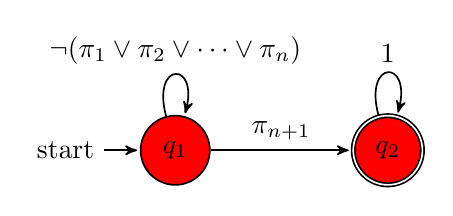
\begin{tikzpicture}[->,>=stealth',shorten >=1pt,auto,node distance=2.7cm,
                    semithick]
  \tikzstyle{every state}=[fill=red,draw=black,text=black]

  \node[initial,state] (A)                    {$q_1$};
  \node[state,accepting]         (B) [right of=A] {$q_2$};

  \path (A) edge              node {$\pi_{n+1}$} (B)
  		(A) edge [loop above] node {$\neg (\pi_1 \lor \pi_2 \lor \dots \lor \pi_n)$} (A)%{$\neg \pi_1 \wedge \neg \pi_2 \wedge \dots \wedge \neg \pi_{n+1}$} (A)
  		(B) edge [loop above] node {$1$} (B);
\end{tikzpicture}
\caption{B\"{u}chi automaton corresponding to $\neg (\pi_1 \lor \pi_2 \lor \dots \lor \pi_n) \U \pi_{n+1}$}
\label{fig:ReachAvoid}
\end{figure}

The B\"{u}chi automaton corresponding to this formula is given in figure \ref{fig:ReachAvoid}. As we can see $d_p(q_1)=1$ and $d_p(q_2)=0$. In this section we will look at the specific formula $\neg \pi_4 \U \pi_5$. The product automaton of this B\"{u}chi automaton combined with the FTS from figure \ref{fig:ftsEx} is shown in figure \ref{fig:reachAvoidProduct}

\begin{figure*}
\centering
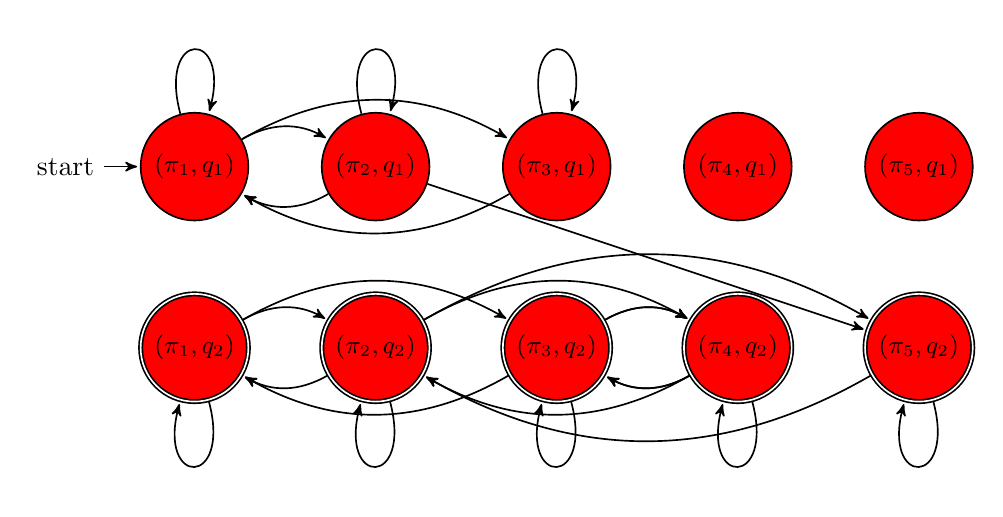
\begin{tikzpicture}[->,>=stealth',shorten >=1pt,auto,node distance=2.3cm,
                    semithick]
  \tikzstyle{every state}=[fill=red,draw=black,text=black]

  \node[initial,state] (A)                    {\small $(\pi_1,q_1)$};
  \node[state]         (B) [ right of=A] {\small $(\pi_2,q_1)$};
  \node[state]         (C) [right of=B] {\small $(\pi_3,q_1)$};
  \node[state]         (D) [right of=C] {\small $(\pi_4,q_1)$};
  \node[state]         (E) [right of=D] {\small $(\pi_5,q_1)$};
  
  \node[state,accepting] 		   (AA)  [below of=A]  {\small $(\pi_1,q_2)$};
  \node[state,accepting]         (BB) [ right of=AA] {\small $(\pi_2,q_2)$};
  \node[state,accepting]         (CC) [right of=BB] {\small $(\pi_3,q_2)$};
  \node[state,accepting]         (DD) [right of=CC] {\small $(\pi_4,q_2)$};
  \node[state,accepting]         (EE) [right of=DD] {\small $(\pi_5,q_2)$};  

  \path (A) edge     [bend left]          (B)
        (B) edge     [bend left]          (A)
        (A) edge     [bend left]         (C)
        (C) edge     [bend left]          (A)
        %(C) edge     [bend left]          (D)
        %(D) edge     [bend left]          (C)
		%(B) edge     [bend left]          (D)
        %(D) edge     [bend left]          (B)
        (B) edge               (EE)
        (DD) edge       [bend left]        (BB)
        (BB) edge        [bend left]       (DD)
        (BB) edge        [bend left]       (AA)
        (AA) edge        [bend left]       (BB)
        (BB) edge        [bend left]       (EE)
        (EE) edge        [bend left]       (BB)
        (DD) edge       [bend left]        (CC)
        (CC) edge        [bend left]       (DD)
        (CC) edge        [bend left]       (DD)
        (DD) edge        [bend left]       (CC)
        (CC) edge        [bend left]       (AA)
        (AA) edge        [bend left]       (CC)
        (A) edge [loop above]  (A)
        (B) edge [loop above]  (B)
        (C) edge [loop above]   (C)
        %(D) edge [loop above]   (D)
        (AA) edge [loop below]  (AA)
        (BB) edge [loop below]  (BB)
        (CC) edge [loop below]  (CC)
        (DD) edge [loop below]   (DD)
        (EE) edge [loop below]   (EE);
\end{tikzpicture}
\caption{Product Automaton for $\neg \pi_4 \U \pi_5$ with Simple FTS}
\label{fig:reachAvoidProduct}
\end{figure*}
Note: in figure \ref{fig:reachAvoidProduct} all nodes have a self loop, which are not included for the sake of the reader.

To find an accepting path, the accepted algorithm starts at the initial node, $(\pi_1,q_1)$, and does a first Dijkstra search to find the optimal path to all the accepting states, $(\pi_i,q_2),$ $\forall i = 1,2,\dots,5$. Then the optimal path back from each of these accepting nodes is computed.  
 
The greedy algorithm does $n+1$ Dijkstra searches, where $n$ is the maximum level of the initial state in the B\"{u}chi automaton. As we can see in figure \ref{fig:ReachAvoid}, $n$ is 1 for all formulas of this form. Therefore the greedy algorithm does one Dijkstra search starting from $(\pi_1,q_1)$ which ends at $(\pi_5,q_2)$. The greedy algorithm will have a slightly faster runtime because it does not find the optimal path back for every accepting node; the greedy algorithm only finds one. 

Because node $q_2$ in automaton \ref{fig:reachAvoidProduct} has a self loop and every region in the simple FTS has a self loop, every accepting state in the product automaton has a self loop. Therefore the cost of the optimal path from any accepting node back to itself is the same i.e.\ 0. This implies that the accepting node that creates the optimal prefix-suffix plan, i.e.\ $q_{f*}'$ in Procedure \ref{optrun}, is the accepting node closest to the initial node. This is the accepting node that the greedy algorithm finds, which in turn implies that both algorithms calculate the same plan. 
%%% CHECK SEMI COLON GRANT

We now investigate the computation time of both algorithms with a case study. So differences in runtime will make themselves apparent, we calculate accepting paths on a larger workspace. The workspace we will use is a grid, 25 units across and 25 units up, a total of 625 equally sized squares. Our robot can move horizontally and vertically, however it cannot move diagonally. Additionally the unit cost of going from any adjacent to another region is 1. The initial position is located at $(0,0)$, region $\pi_1$ is located at (2,24), region $\pi_2$ is located at (12,12), and region $\pi_3$ is located at (20,15). This workspace is seen in figure \ref{fig:workspace}.

\begin{figure}[!htb]
\centering
\includegraphics[scale=0.8]{workspace.eps}
\label{fig:workspace}
\caption{Workspace 1}
\end{figure}


The output from the accepted algorithm is \\


\begin{minipage}{\textwidth}
\begingroup
\fontsize{9pt}{12pt}\selectfont
\begin{lstlisting}
Accepted Algorithm
==================
accepted_plan done within 0.02s: precost 35.00, sufcost 0.00
------------------------------
the prefix of plan **states**:
[((0, 0, 1), 'None'), ((1, 0, 1), 'None'), ((2, 0, 1), 'None'), ((3, 0, 1), 'None'), ((3, 1, 1), 'None'), ((4, 1, 1), 'None'), ((5, 1, 1), 'None'), ((6, 1, 1), 'None'), ((6, 2, 1), 'None'), ((6, 3, 1), 'None'), ((6, 4, 1), 'None'), ((6, 5, 1), 'None'), ((7, 5, 1), 'None'), ((8, 5, 1), 'None'), ((8, 6, 1), 'None'), ((9, 6, 1), 'None'), ((10, 6, 1), 'None'), ((10, 7, 1), 'None'), ((10, 8, 1), 'None'), ((10, 9, 1), 'None'), ((11, 9, 1), 'None'), ((12, 9, 1), 'None'), ((12, 10, 1), 'None'), ((13, 10, 1), 'None'), ((14, 10, 1), 'None'), ((14, 11, 1), 'None'), ((15, 11, 1), 'None'), ((16, 11, 1), 'None'), ((17, 11, 1), 'None'), ((18, 11, 1), 'None'), ((19, 11, 1), 'None'), ((19, 12, 1), 'None'), ((20, 12, 1), 'None'), ((20, 13, 1), 'None'), ((20, 14, 1), 'None'), ((20, 15, 1), 'None'), ((20, 15, 1), 'None')]
the suffix of plan **states**:
[((20, 15, 1), 'None'), ((20, 15, 1), 'None')]
------------------------------
the prefix of plan **actions**:
[(0, 0, 1), (1, 0, 1), (2, 0, 1), (3, 0, 1), (3, 1, 1), (4, 1, 1), (5, 1, 1), (6, 1, 1), (6, 2, 1), (6, 3, 1), (6, 4, 1), (6, 5, 1), (7, 5, 1), (8, 5, 1), (8, 6, 1), (9, 6, 1), (10, 6, 1), (10, 7, 1), (10, 8, 1), (10, 9, 1), (11, 9, 1), (12, 9, 1), (12, 10, 1), (13, 10, 1), (14, 10, 1), (14, 11, 1), (15, 11, 1), (16, 11, 1), (17, 11, 1), (18, 11, 1), (19, 11, 1), (19, 12, 1), (20, 12, 1), (20, 13, 1), (20, 14, 1), (20, 15, 1), 'None', 'None']
the suffix of plan **actions**:
['None', 'None']
full construction and synthesis done within 0.11s
\end{lstlisting}
\endgroup
\end{minipage} \\ \\


The output of the algorithm is structured as follows: the time taken to calculate the path, the cost of the prefix, and the cost of the suffix are given at the top of the output. The follow sequence of "states" can be thought of as the result of the labelling function \ref{defDLF}, and actions can be thought of the labels of the transition of the B\"uchi automaton. The \texttt{full construction and synthesis} includes the time taken to initialize and construct the graph, thus it is larger than the first time given. The initialization and construction of the graph almost always takes the majority of time. For the rest of this report, the calculated paths will appear in the appendix.% for the ease of the reader.

The greedy algorithm outputs the same plan marginally faster. \\


\begin{minipage}{\textwidth}
\begingroup
\fontsize{9pt}{12pt}\selectfont
\begin{lstlisting}
Greedy Algorithm
===============
greedy_plan done within 0.01s: precost 35.00, sufcost 0.00
...
full construction and synthesis done within 0.10s 
\end{lstlisting}
\endgroup
\end{minipage} \\ \\


%As we can see, our algorithm computed the same path in about the same time.%seconds. This may seem weird because we have shown that our algorithm does the same calculation when finding a path from the initial node to an accepting node. The difference is that for each accepting node, a Dijkstra search is performed. In this example, there are 625 accepting states (the number of states in the FTS times the number of states in the B\"uchi automaton). The function \texttt{dijkstra\_predecessor\_and\_distance} from \cite{schult08} is used to calculate the shortest path back to an accepting node. 
\section{Sequencing}
Sequencing is the behaviour of visiting regions $\pi_1,\pi_2,\dots,\pi_n$ in that order. One example of a formula of this type is $\diamond (\pi_3 \land  \diamond \pi_5)$ and the corresponding B\"uchi automaton is shown in figure \ref{fig:seq}. We note that this automaton is only applicable because of the partition we defined earlier in Definition \ref{def:PM} which makes it impossible for $\pi_i$ and $\pi_j$ to be true at the same time if $i\neq j$. The LTL2BA tool \cite{ltlbuchiwebsite} that is used generates an automaton with an edge from $q_1$ to $q_3$ labelled $\pi_3 \&\& \pi_5 $. This transition is impossible so we take it out before calculating the distances. The greedy algorithm would not work if every state in the B\"uchi automaton had a distance of 1 and the accepting states had a distance of 0. The product automaton of formula $\diamond (\pi_3 \wedge \diamond \pi_5)$ the simple FTS is shown in figure \ref{fig:Sequencing}


\begin{figure}
\centering
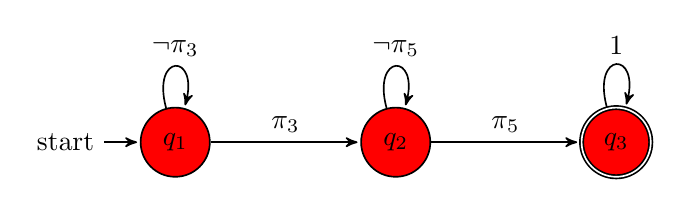
\begin{tikzpicture}[->,>=stealth',shorten >=1pt,auto,node distance=2.8cm,
                    semithick]
  \tikzstyle{every state}=[fill=red,draw=black,text=black]

  \node[initial,state] (A)                    {$q_1$};
  %\node[state] (B)                    [right of=A]{$q_2$};
  \node[state] (B)                    [right of=A]{$q_2$};
  \node[state,accepting]         (C) [right of=B] {$q_3$};

  \path (A) edge              node {$\pi_{3}$} (B)
  		(A) edge [loop above] node {$\neg \pi_3$} (A)
  		(B) edge [loop above] node {$\neg \pi_5$} (B)
  		(B) edge              node {$\pi_{5}$} (C)
  		(C) edge [loop above] node {$1$} (C);
%  		(C) edge              node {$\pi_{3}$} (D)
 % 		(D) edge [loop above] node {$1$} (D);
\end{tikzpicture}
\caption{B\"uchi Automaton Corresponding to $  \diamond(\pi_3 \land \diamond \pi_5)$}
\label{fig:seq}
\end{figure}

\begin{figure*}
\centering
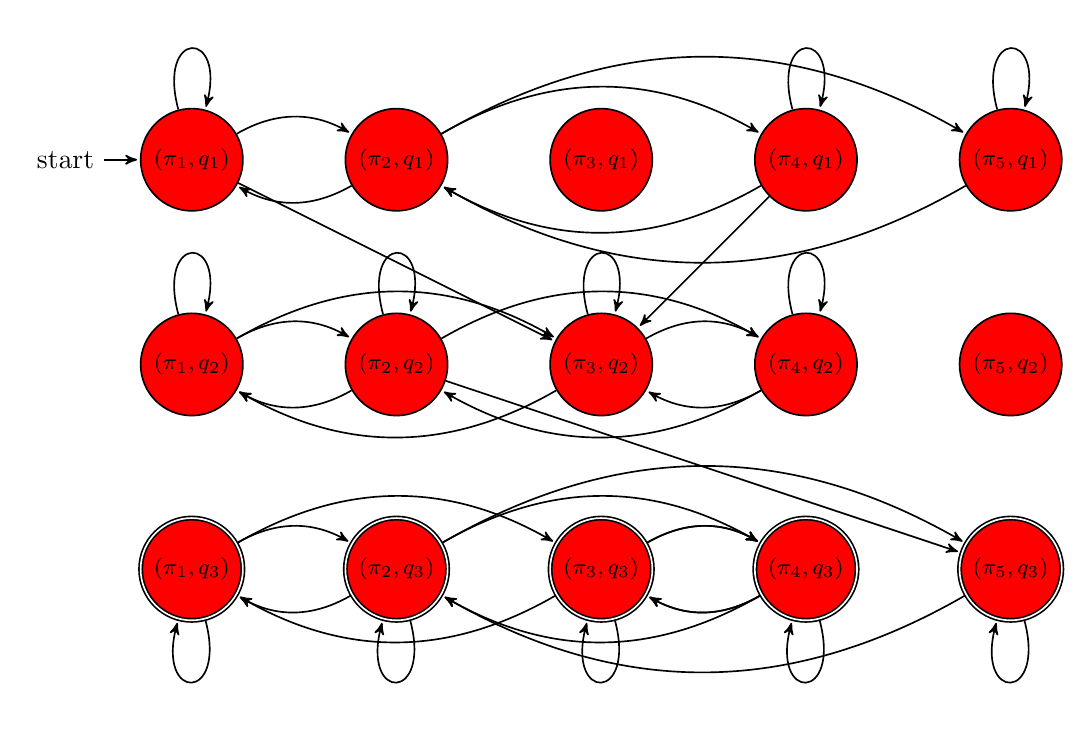
\begin{tikzpicture}[->,>=stealth',shorten >=1pt,auto,node distance=2.6cm,
                    semithick]
  \tikzstyle{every state}=[fill=red,draw=black,text=black]

  \node[initial,state] (A)                    {\footnotesize $(\pi_1,q_1)$};
  \node[state]         (B) [ right of=A] {\footnotesize $(\pi_2,q_1)$};
  \node[state]         (C) [right of=B] {\footnotesize $(\pi_3,q_1)$};
  \node[state]         (D) [right of=C] {\footnotesize $(\pi_4,q_1)$};
  \node[state]         (E) [right of=D] {\footnotesize $(\pi_5,q_1)$};
  
  \node[state] 		   (AA)  [below of=A]  {\footnotesize $(\pi_1,q_2)$};
  \node[state]         (BB) [ right of=AA] {\footnotesize $(\pi_2,q_2)$};
  \node[state]         (CC) [right of=BB] {\footnotesize $(\pi_3,q_2)$};
  \node[state]         (DD) [right of=CC] {\footnotesize $(\pi_4,q_2)$};
  \node[state]         (EE) [right of=DD] {\footnotesize $(\pi_5,q_2)$};
  
  \node[state,accepting] 		   (AAA)  [below of=AA]  {\footnotesize $(\pi_1,q_3)$};
  \node[state,accepting]         (BBB) [ right of=AAA] {\footnotesize $(\pi_2,q_3)$};
  \node[state,accepting]         (CCC) [right of=BBB] {\footnotesize $(\pi_3,q_3)$};
  \node[state,accepting]         (DDD) [right of=CCC] {\footnotesize $(\pi_4,q_3)$};
  \node[state,accepting]         (EEE) [right of=DDD] {\footnotesize $(\pi_5,q_3)$};
  

  \path (A) edge     [bend left]          (B)
        (B) edge     [bend left]          (A)
        %(A) edge     [bend left]         (C)
        %(C) edge     [bend left]          (A)
        %(C) edge		[bend left] 		(D)
        %(D) edge 		[bend left]      (C)
        (A) edge               (CC)
        %(BB) edge               (EEE)
        (BB)	edge			[loop above] (BB)
        (AA)	edge			[loop above] (AA)
        (CC)	edge			[loop above] (CC)
        (DD)	edge			[loop above] (DD)
        (A)	edge			[loop above] (A)
        (E)	edge			[loop above] (E)
        (D)	edge			[loop above] (D)
        (AAA)	edge			[loop below] (AAA)
        (BBB)	edge			[loop below] (BBB)
        (CCC)	edge			[loop below] (CCC)
        (DDD)	edge			[loop below] (DDD)
        (EEE)	edge			[loop below] (EEE)
        (D) edge               (CC)
        (B) edge       [bend left]        (E)
        (E) edge       [bend left]        (B)
        (B) edge       [bend left]        (D)
        (D) edge       [bend left]        (B)
        (BB) edge 			(EEE)
%        (EE) edge			[bend left]		(BB)
        (DD) edge       [bend left]        (BB)
        (BB) edge        [bend left]       (DD)
        (BB) edge        [bend left]       (AA)
        (AA) edge        [bend left]       (BB)
        (CC) edge        [bend left]       (AA)
        (AA) edge        [bend left]       (CC)
        (CC) edge        [bend left]       (DD)
        (DD) edge        [bend left]       (CC)
        
        (DDD) edge       [bend left]        (BBB)
        (BBB) edge        [bend left]       (DDD)
        (BBB) edge        [bend left]       (AAA)
        (AAA) edge        [bend left]       (BBB)
        (BBB) edge        [bend left]       (EEE)
        (EEE) edge        [bend left]       (BBB)
        (DDD) edge       [bend left]        (CCC)
        (CCC) edge        [bend left]       (DDD)
        (CCC) edge        [bend left]       (DDD)
        (DDD) edge        [bend left]       (CCC)
        (CCC) edge        [bend left]       (AAA)
        (AAA) edge        [bend left]       (CCC);
\end{tikzpicture}
\caption{Product Automaton for $\diamond (\pi_4 \wedge \diamond \pi_5)$ with Simple FTS}
\label{fig:Sequencing}
\end{figure*}

We look at how the two algorithms will search this product automaton to find an accepting path. The accepted algorithm starts at the initial node $(\pi_1,q_1)$ and in the first step searches the nodes connected to $(\pi_1,q_1)$ i.e.\ $(\pi_2,q_1)$ and $(\pi_3,q_2)$. In the next step it searches $(\pi_4,q_1)$, $(\pi_5,q_1)$, $(\pi_1,q_2)$, $(\pi_4,q_2)$. Next it searches $(\pi_2,q_2)$ and then $(\pi_5,q_3)$. Even though $(\pi_5,q_3)$ is an accepting state, the accepted algorithm continues the search because it has to find the shortest path to \textit{all} accepting nodes. The next step it searches $(\pi_2,q_3)$, then $(\pi_1,q_3)$ and $(\pi_4,q_3)$ and finally $(\pi_3,q_3)$. After this, it finds the shortest path from all accepting nodes back to themselves. Again every, accepting node has a self loop so all the accepting nodes have a suffix cost of 0. 



The greedy algorithm also starts at $(\pi_1,q_1)$ and in the first step searches $(\pi_2,q_1)$ and $(\pi_3,q_2)$. The greedy algorithm notices that the current level is 2, and $(\pi_3,q_2)$ is on level 1. Because the level of $(\pi_3,q_2)$ is 1 below the current level, the greedy algorithm finishes the Dijkstra search and starts another Dijkstra search beginning at $(\pi_3,q_2)$. In the first step, $(\pi_1,q_2)$ and $(\pi_4,q_2)$ are searched. It will then do another step and search $(\pi_2,q_2)$. Finally in the third step, it searches $(\pi_5,q_3)$. It notices $(\pi_5,q_3)$ is an accepting state and finishes the search. It then finds the optimal path from $(\pi_5,q_3)$ back to itself.

We run both algorithms with the formula $\diamond (\pi_1 \land \diamond(\pi_2 \land \diamond \pi_3))$ and Workspace 1 in figure \ref{fig:workspace}. The output of the accepted algorithm is \\


\begin{minipage}{\textwidth}
\begingroup
\fontsize{9pt}{12pt}\selectfont
\begin{lstlisting}
Accepted Algorithm
==================
accepted_plan done within 0.04s: precost 62.00, sufcost 0.00
...
full construction and synthesis done within 0.19s 
\end{lstlisting}
\endgroup
\end{minipage} \\ \\


The greedy algorithm computed the same path, with an output of \\


\begin{minipage}{\textwidth}
\begingroup
\fontsize{9pt}{12pt}\selectfont
\begin{lstlisting}
Greedy Algorithm
================
greedy_plan done within 0.02s: precost 62.00, sufcost 0.00
...
full construction and synthesis done within 0.17s 
\end{lstlisting}
\endgroup
\end{minipage} \\ \\


As we can see, the plan synthesis took the greedy algorithm half as long; 0.02 seconds compared to 0.04 seconds. We take a look at what causes the increased time. 

\begin{figure}[!htb]
\centering
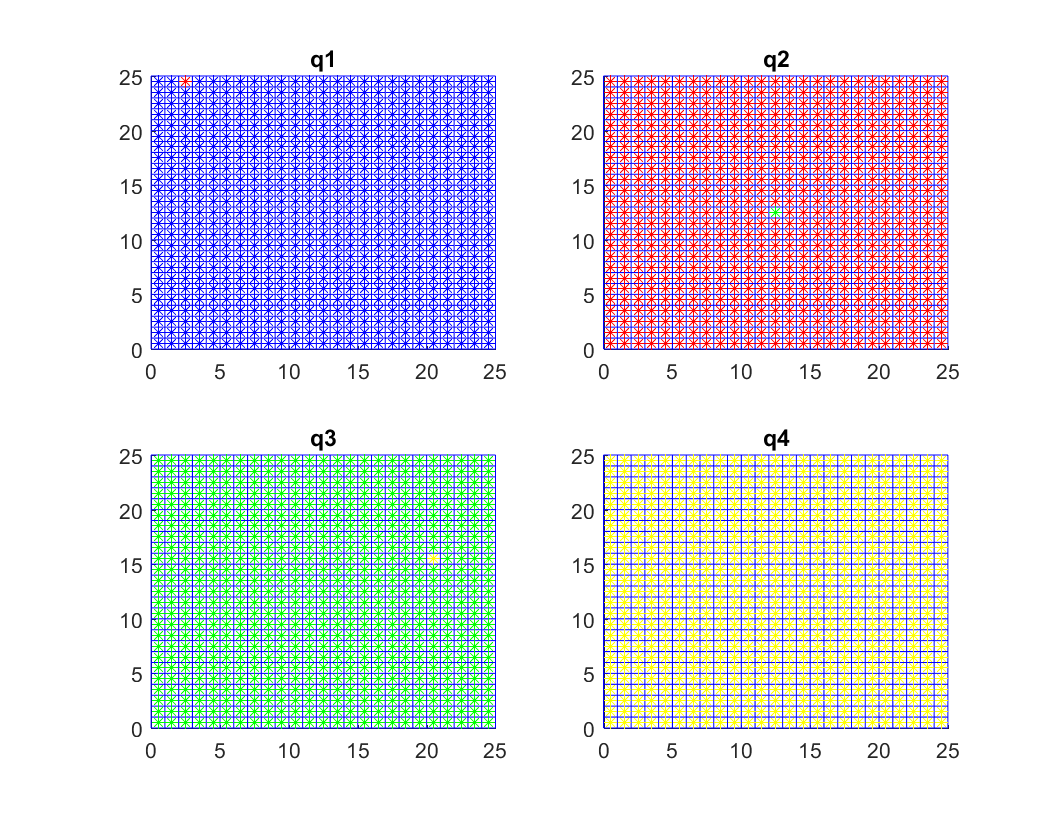
\includegraphics[scale=0.7]{acceptedPlot}
\label{fig:animAccept}
\caption{Nodes searched with the accepted algorithm}
\end{figure}

\begin{figure}[!htb]
\centering
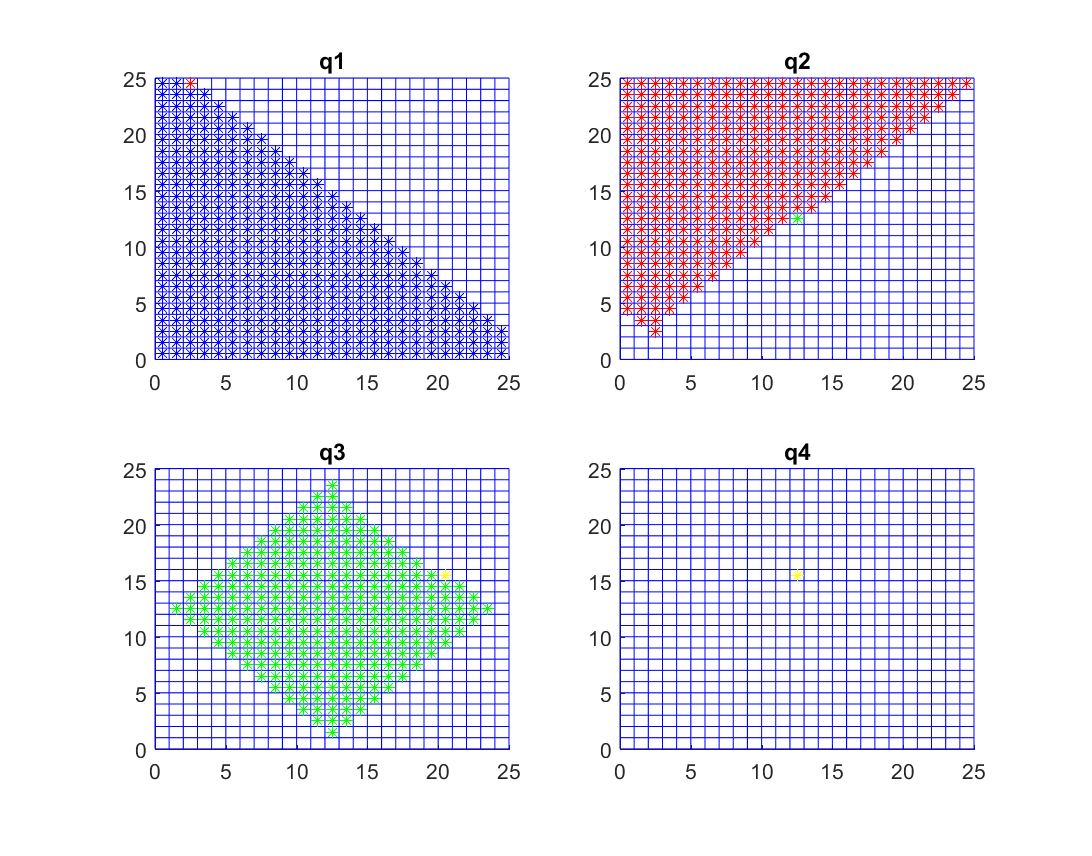
\includegraphics[scale=0.7]{ourPlot}
\label{fig:animOur}
\caption{Nodes searched with the greedy algorithm}
\end{figure}

Figure \ref{fig:animAccept} shows the states searched with the accepted algorithm and figure \ref{fig:animOur} shows the states searched with the greedy algorithm. Each figure shows a representation of the product automaton. The graph can be thought of as the discretization of the workspace, and there are four corresponding to the four states in the B\"uchi automaton. Any square filled in with blue, red, green, or yellow has been visited, all others have not. As we can see, the greedy algorithm searches a significantly smaller number of nodes, while the accepted algorithm searches every node.

The FTS has 625 and the B\"uchi automaton has four states, which implies the product automaton has 2500 states. The accepted algorithm does one Dijkstra search from the initial node to each of the 2499 other nodes, and then computes the suffix cost for each of the 625 accepting nodes. The algorithm then chooses which combination out of the 625 choices makes the shortest overall run. 

The level of the initial node is three, so the greedy algorithm does three Dijkstra searches; one for each level and one for the accepted node back to itself. To find an accepting node, the the first search searches through 326 nodes, the second 266 nodes, and the third 587 nodes. The last search simply finds the path from the accepting node back to itself, which is a self loop. Thus the greedy algorithm searches 1179 nodes compared to 2500 nodes.  
%Check how many nodes are searched with both algorithms, and show time difference.

Because there is only one way down at each level, the concatenation of the locally optimal paths will be the globally optimal path. Then the advantage that the greedy algorithm has over the accepted algorithm is that the accepted algorithm will search through more extraneous nodes. Because all accepting nodes have the same suffix cost, the optimal accepting node will be the one closest to the initial node. This is the one the greedy algorithm finds. Thus the greedy algorithm is guaranteed find the optimal path in a shorter amount of time than the accepted algorithm.


\section{Coverage}
A coverage formula represents the statement visit $\pi_1, \pi_2, \dots, \pi_n$ in any order, and is of the form $\varphi = \diamond \pi_1 \wedge \diamond \pi_2 \wedge \dots \wedge \diamond \pi_n$. We show the B\"uchi automaton corresponding to the formula $\diamond \pi_1 \wedge \diamond \pi_2 \wedge \diamond \pi_3$ in figure \ref{fig:buchCov}

\begin{figure}
\centering
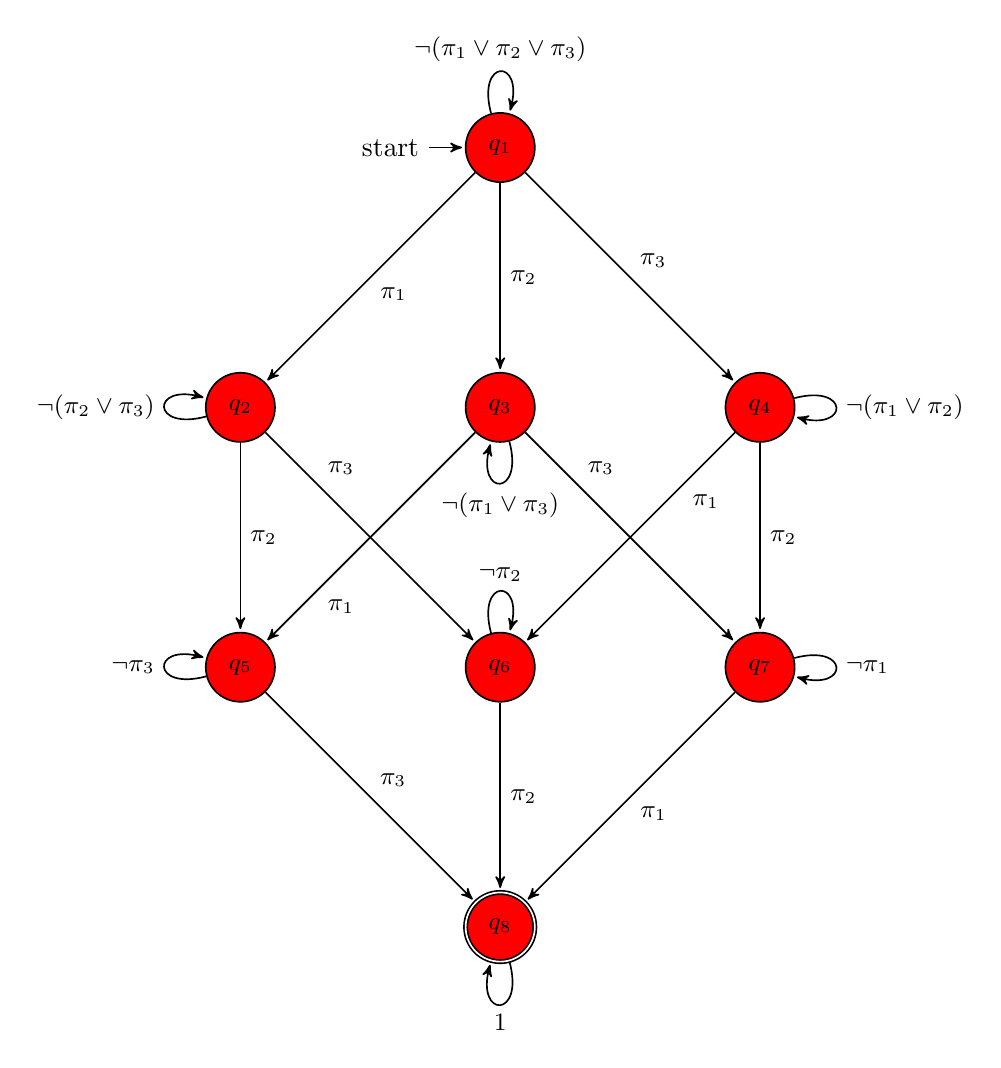
\begin{tikzpicture}[->,>=stealth',shorten >=1pt,auto,node distance=3.3cm,
                    semithick]
  \tikzstyle{every state}=[fill=red,draw=black,text=black]

  \node[initial,state] (A)                    {\small $q_1$};
  \node[state] (C)                    [below of=A]{\small $q_3$};
  \node[state] (D)                    [right of=C]{\small $q_4$};
  \node[state]         (B) [left of=C] {\small $q_2$};
  \node[state] (E) 					[below of=B]{\small $q_5$};
   \node[state] (F) 					[below of=C]{\small $q_6$};
   \node[state] (G) 					[below of=D]{\small $q_7$};
   \node[accepting,state] (H) 					[below of=F]{\small $q_8$};
  

  \path (A) edge              node {\small $\pi_{1}$} (B)
   (A) edge              node {\small $\pi_{2}$} (C)
   (A) edge              node {\small $\pi_{3}$} (D)
   (B) edge              node {\small $\pi_{2}$} (E)
   (B) edge              node [near start] {\small $\pi_{3}$} (F)
   (C) edge              node [near end] {\small $\pi_{1}$} (E)
   (E) edge              node {\small $\pi_{3}$} (H)
   (F) edge              node {\small $\pi_{2}$} (H)
   (G) edge              node {\small $\pi_{1}$} (H)
   (D) edge              node {\small $\pi_{2}$} (G)
   (A) edge      [loop above]        node {\small $\neg (\pi_1 \lor \pi_{2} \lor\pi_3)$} (A)
   (B) edge      [loop left]        node {\small $\neg (\pi_{2} \lor \pi_3)$} (B)
   (C) edge      [loop below]        node {\small $\neg( \pi_1 \lor \pi_3)$} (C)
   (D) edge      [loop right]        node {\small $\neg (\pi_1 \lor \pi_{2}) $} (A)
   (E) edge      [loop left]        node {\small $\neg  \pi_3$} (E)
   (F) edge      [loop above]        node {\small $\neg  \pi_2$} (F)
   (G) edge      [loop right]        node {\small $\neg  \pi_1$} (G)
   (H) edge      [loop below]        node {\small $1$} (H)
   (D) edge              node [near start] {\small $\pi_{1}$} (F)
   (C) edge              node [near start] {\small $\pi_{3}$} (G);
\end{tikzpicture}
\caption{B\"uchi Automaton Corresponding to $\diamond \pi_1 \wedge \diamond \pi_2 \wedge \diamond \pi_3$}
\label{fig:buchCov}
\end{figure}

We can see that to get to the accepting node, we have to choose which node to go to first, and then which node to go to second (the third node we then have to visit is already decided). So, there are 6 possible paths to take from the initial node, $q_1$ to accepting state $q_8$. This is true in the product automaton too, if we only consider the option of taking the optimal path between nodes. 

The accepted algorithm will search through the whole product automaton and will then choose the order that produces the global minimum. The greedy algorithm on the other hand will first choose $\pi_i$ which is the closest to the initial node. From there, it will choose $\pi_j$ which is closest to $\pi_i$ out of the two that have not been visited yet. Thus the greedy algorithm may not compute the globally optimal path on a coverage formula. It will however compute an accepting path, with a bound on the cost of the greedy path in terms of the cost of the optimal path. 

To prove this cost bound, we first show that this path corresponds to the one generated by the nearest neighbour approach to the travelling salesperson problem. Next we provide the bound on the cost of our path based on the worst case ratio of the nearest neighbour path to the optimal path given by Rosendrantz, Stearns, and Lewis \cite{rosenkrantz74}. 

%This problem is NP-hard, 
\subsection{Travelling Salesperson Problem}
The travelling salesperson problem is stated in layman's terms as finding the shortest path for a salesperson to take such that he passes through a given set of cities and then returns back home at the end. This problem has been studied extensively and many algorithms and heuristics exist for finding an approximate solution. One very simple algorithm to do this is called the nearest neighbour algorithm. It says from the starting city, pick the closest city to be the next stop. From there, pick the next closest city not including the starting city, and so on. If there is a tie in the next closest neighbour, the next node can be decided arbitrarily. This is exactly what the greedy algorithm does given a coverage formula; the first Dijkstra search finds the closest node, we start another search from that node and so on. 

To formulate our problem as a travelling salesman problem we use the idea of a dummy node from the computer wiring example in \cite{lenstra75}. In the example, a computer interface is being designed at the Institute for Nuclear Physical Research in Amsterdam. An interface is made up of several modules, with multiple pins on each module. A given subset of pins has to be interconnnected by wires, and at most two wires can be connected to any pin. For obvious reasons, it is desirable to minimize the amount of wire used. They show that this problem can be formulated as a travelling salesperson problem. The only difference between this problem and a travelling salesman problem is that in the travelling salesman problem, the salesman must return home at the end. This is not true in this problem. It is also not true in our problem, we only need to pass through $\pi_1$, $\pi_2$ and $\pi_3$ and there is no need to return to the starting state after we do this. To formulate this problem as a travelling salesperson problem, they set $P$ to be the set of pins to be interconnected, and $c_{ij}$ to be the distance between pin $i$ and pin $j$. They then introduce a dummy node $*$ that is a distance 0 from all the other nodes i.e.\ $c_{i*} = c_{*i} = 0$ for all i. Then the corresponding problem is solving the travelling salesperson problem on the set of nodes $N=P \cup \{*\}$. 

For our problem, we set $c_{ij}=d(\pi_i , \pi_j)$, for $i,j=0,1,2,3$ where the initial state is from now on known as $\pi_0$, to be the shortest path our robot can take from $\pi_i$ to $\pi_j$. When introducing the dummy node, we must preserve the the triangle inequality for a proof of a worst case scenario bound we will provide later on. To do this, we cannot have the dummy node be distance 0 from the other nodes. Indeed, if $c_{i*} = c_{*i} = 0 $ the triangle inequality would be violated because $c_{i*} + c_{*j} = 0 \leq c_{ij}$.

We can represent the relationship between the regions in our graph with the following \textit{complete} subgraph, shown in figure \ref{fig:completeGraph}. A complete graph is an undirected graph in which every pair of vertices is connected by an edge. 
\begin{figure}
\centering
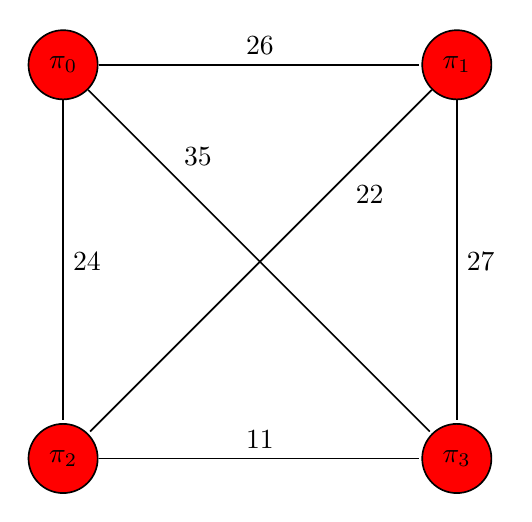
\begin{tikzpicture}[-,>=stealth',shorten >=1pt,auto,node distance=5cm,
                    semithick]
  \tikzstyle{every state}=[fill=red,draw=black,text=black]

  \node[state] (A)                    {$\pi_0$};
  \node[state] (B)                    [right of=A]{$\pi_1$};
  \node[state] (C)                    [below of=A]{$\pi_2$};
  \node[state]         (D) [right of=C] {$\pi_3$};

  \path (A) edge              node {$26$} (B)
  		(A) edge 			 node {$24$} (C)
  		(A) edge              node [near start] {$35$} (D)
  		(B) edge 				node [near start] {$22$} (C)
  		(B) edge              node {$27$} (D)
  		(C) edge				node {$11$} (D);
\end{tikzpicture}
\caption{Complete Graph between Regions of Interest}
\label{fig:completeGraph}
\end{figure}

For the distances, we use the so called \textit{Manhattan distance}, i.e.\ \\ $d((x_1,y_1),(x_2,y_2)) = |x_1 - x_2| +| y_1 - y_2|$ because our robot can only move horizontally and vertically, not diagonally. Given the weights between the vertices, we easily see that the path that the greedy algorithm will take is shown in figure \ref{fig:pathOnComplete}. The cost of this path is 62. This is not the optimal path however, which is shown in figure \ref{fig:optcompleteGraph} and has a cost of 59.

\begin{figure}
\centering
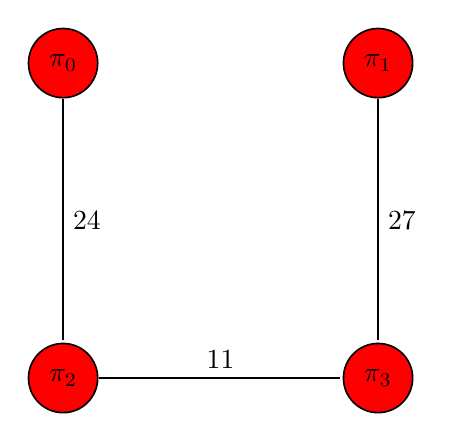
\begin{tikzpicture}[-,>=stealth',shorten >=1pt,auto,node distance=4cm,
                    semithick]
  \tikzstyle{every state}=[fill=red,draw=black,text=black]

  \node[state] (A)                    {$\pi_0$};
  \node[state] (B)                    [right of=A]{$\pi_1$};
  \node[state] (C)                    [below of=A]{$\pi_2$};
  \node[state]         (D) [right of=C] {$\pi_3$};

  \path (A) edge 			 node {$24$} (C)
  		(B) edge              node {$27$} (D)
  		(C) edge				node {$11$} (D);
\end{tikzpicture}
\caption{Nearest Neighbour Path}
\label{fig:pathOnComplete}
\end{figure}


\begin{figure}
\centering
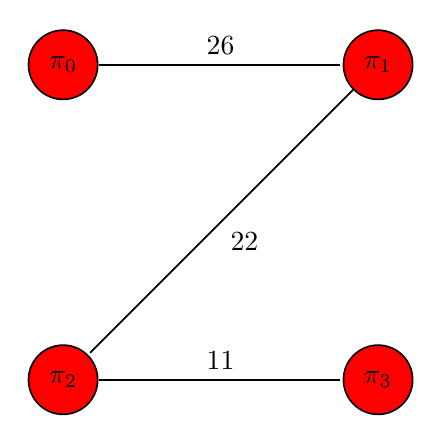
\begin{tikzpicture}[-,>=stealth',shorten >=1pt,auto,node distance=4cm,
                    semithick]
  \tikzstyle{every state}=[fill=red,draw=black,text=black]

  \node[state] (A)                    {$\pi_0$};
  \node[state] (B)                    [right of=A]{$\pi_1$};
  \node[state] (C)                    [below of=A]{$\pi_2$};
  \node[state]         (D) [right of=C] {$\pi_3$};

  \path (A) edge              node {$26$} (B)
  		%(A) edge 			 node {$24$} (C)
  		%(A) edge              node {$35$} (D)
  		(B) edge 				node {$22$} (C)
  		%(B) edge              node {$27$} (D)
  		(C) edge				node {$11$} (D);
\end{tikzpicture}
\caption{Optimal Path}
\label{fig:optcompleteGraph}
\end{figure}


Because we have to make sure that the dummy node does not change the order that the greedy algorithm and the nearest neighbour algorithm take we have to set the distance of the dummy node from every other node to be $\max_{i,j} c_{ij} $ where $c_{ij}$ is the distance between the nodes in the complete subgraph in figure \ref{fig:completeGraph}. In our case, this is 35, the path between $\pi_0$ and $\pi_3$. This insures that the path taken by the greedy algorithm is the same as the nearest neighbour algorithm because the dummy node will be the last node to be visited. Thus, the only time where it is a possibility that the nearest neighbour algorithm goes to the dummy node i.e.\ when the next node is $\max_{i,j} c_{ij}$ from the current node, is when and if we are faced with the only choice being take the maximum path $ \max_{i,j} \hspace{0.1cm} c_{i,j}$ to $\pi_j$ or to go to the dummy node. We say we to go to $\pi_j$ because the ties can be broken arbitrarily. In any other case, the nearest neighbour path will choose to go to a node where the cost is $c_{i',j'} < c_{i,j}$. We show the new subgraph in figure \ref{fig:completeDummy}

\begin{figure}
\centering
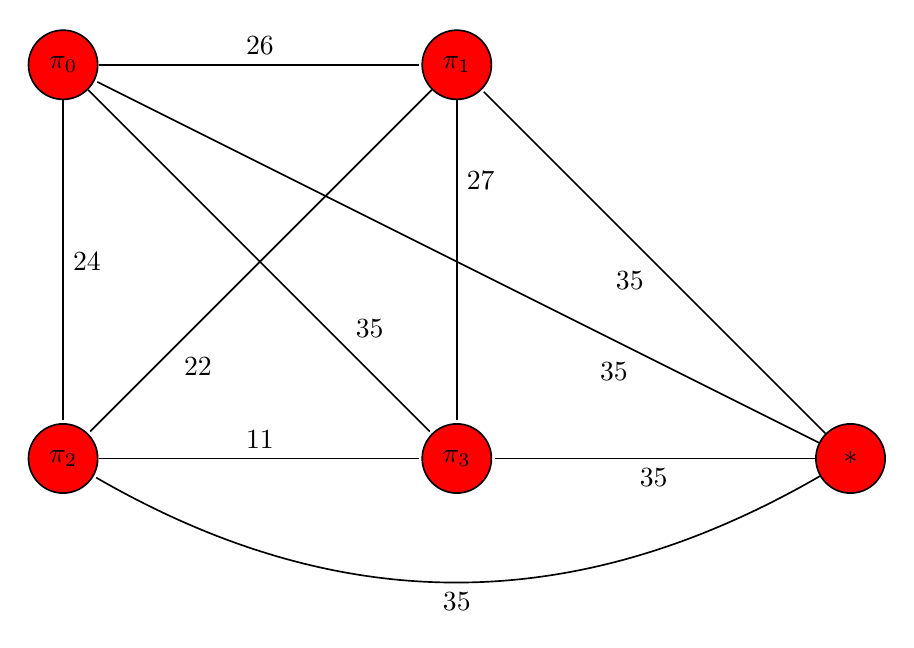
\begin{tikzpicture}[-,>=stealth',shorten >=1pt,auto,node distance=5cm,
                    semithick]
  \tikzstyle{every state}=[fill=red,draw=black,text=black]

  \node[state] (A)                    {$\pi_0$};
  \node[state] (B)                    [right of=A]{$\pi_1$};
  \node[state] (C)                    [below of=A]{$\pi_2$};
  \node[state]         (D) [right of=C] {$\pi_3$};
  \node[state] (E)			[right of = D] {$*$}; 

  \path (A) edge              node {$26$} (B)
  		(A) edge 			 node {$24$} (C)
  		(A) edge              node [near end] {$35$} (D)
  		(B) edge 				node [near end] {$22$} (C)
  		(B) edge              node [near start] {$27$} (D)
  		(C) edge				node {$11$} (D)
  		(E) edge 				node {$35$} (D)
  		(E) edge 				[bend left] node {$35$} (C)
  		(E) edge 				node {$35$} (B)
  		(E) edge 				node [near start] {$35$} (A);
\end{tikzpicture}
\caption{Complete Subgraph with Dummy Node}
\label{fig:completeDummy}
\end{figure}

The path that the nearest neighbour algorithm takes in this situation is given in figure \ref{fig:NearNeigDummy}, which gives a total cost of 132. Again, this is not the optimal solution. The optimal solution is shown in figure \ref{fig:optDummy} and has a cost of 129.

\begin{figure}
\centering
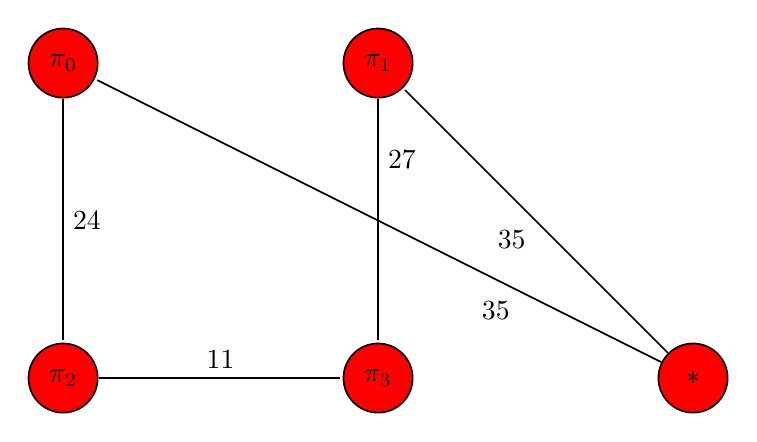
\begin{tikzpicture}[-,>=stealth',shorten >=1pt,auto,node distance=4cm,
                    semithick]
  \tikzstyle{every state}=[fill=red,draw=black,text=black]

  \node[state] (A)                    {$\pi_0$};
  \node[state] (B)                    [right of=A]{$\pi_1$};
  \node[state] (C)                    [below of=A]{$\pi_2$};
  \node[state]         (D) [right of=C] {$\pi_3$};
  \node[state] (E)			[right of = D] {$*$}; 

  \path (A) edge 			 node {$24$} (C)
  		%(A) edge              node {$35$} (D)
  		%(B) edge 				node {$22$} (C)
  		(B) edge              node [near start] {$27$} (D)
  		(C) edge				node {$11$} (D)
  		%(E) edge 				node {$35$} (D)
  		%(E) edge 				[bend left] node {$35$} (C)
  		(E) edge 				node {$35$} (B)
  		(E) edge 				node [near start] {$35$} (A);
\end{tikzpicture}
\caption{Nearest Neighbour Path with Dummy Node}
\label{fig:NearNeigDummy}
\end{figure}


\begin{figure}
\centering
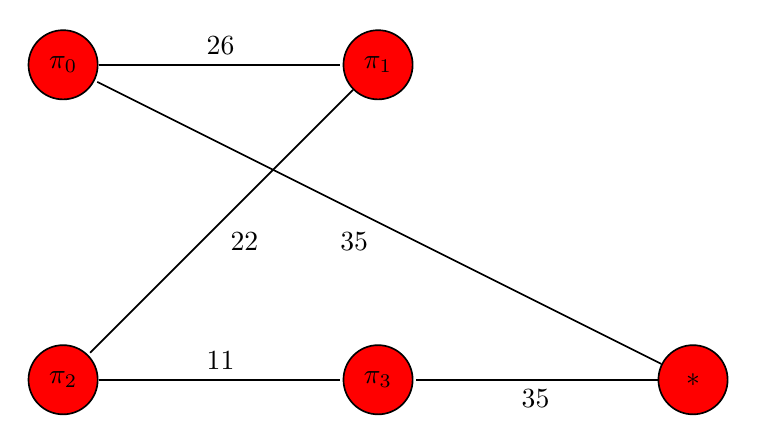
\begin{tikzpicture}[-,>=stealth',shorten >=1pt,auto,node distance=4cm,
                    semithick]
  \tikzstyle{every state}=[fill=red,draw=black,text=black]

  \node[state] (A)                    {$\pi_0$};
  \node[state] (B)                    [right of=A]{$\pi_1$};
  \node[state] (C)                    [below of=A]{$\pi_2$};
  \node[state]         (D) [right of=C] {$\pi_3$};
  \node[state] (E)			[right of = D] {$*$}; 

  \path (A) edge			node {$26$} (B)
  		%(A) edge 			 node {$24$} (C)
  		%(A) edge              node {$35$} (D)
  		(B) edge 				node {$22$} (C)
  		%(B) edge              node {$27$} (D)
  		(C) edge				node {$11$} (D)
  		(E) edge 				node {$35$} (D)
  		%(E) edge 				[bend left] node {$35$} (C)
  		%(E) edge 				node {$35$} (B)
  		(E) edge 				node {$35$} (A);
\end{tikzpicture}
\caption{Optimal Path with Dummy Node}
\label{fig:optDummy}
\end{figure}


\subsection{Cost Bound}

It has been shown \cite{rosenkrantz74} that for an n-node travelling salesperson problem which satisfies the triangle inequality i.e.\ $d(i,j) + d(j,k) \geq d(i,k)$ for all $i,j,$ and $k$ where $d(i,j)$ is the nonnegative distance between nodes $i$ and $j$, 
\begin{align*}
\text{NEARNEIBR} \leq (\frac{1}{2} \lceil \log(n) \rceil + \frac{1}{2})\text{OPTIMAL}
\end{align*}
where NEARNEIBR is the cost of the path generated by the nearest neighbour algorithm and OPTIMAL is the cost of the optimal path. 

Our values do indeed satisfy this inequality
\begin{align*}
\text{NEARNEIBR} &\leq (\frac{1}{2} \lceil \log(n) \rceil + \frac{1}{2})\text{OPTIMAL} \\
132 &\leq (\frac{1}{2} \lceil \log(5) \rceil + \frac{1}{2})129 \\
132 &\leq 258 
\end{align*}
We also see that it is very conservative worst case bound and we will likely do much better.

We provide a proof of
\begin{align}
\dfrac{\text{NEARNEIBR}}{\text{OPTIMAL}} \leq \frac{1}{2} \lceil \log(n) \rceil + \frac{1}{2}
\end{align}
which can be found in \cite{rosenkrantz74}. 
Proof:
We begin by proving 
\begin{align}
\text{OPTIMAL} \geq 2 \sum^{\min(2k,n)}_{i=k+1} l_i \label{eq:showFirst}
\end{align}
for all $k$, $0\leq k \leq n$. 
Let $l_i$ be the length of the $i^{th}$ largest edge in the path obtained by the nearest neighbour algorithm. For each $i$, $0 \leq i \leq n$, let $a_i$ be the node \textit{onto which} the $i^{th}$ largest edge is added to (that would be the edge with length $l_i$). Let $H$ be the complete subgraph defined on the set of nodes $\{a_i \hspace{0.1cm} | \hspace{0.1cm} 1 \leq i \leq min(2k,n)\}$.

Now, let $T$ be the path in $H$ which visits the nodes of $H$ in the same order as these nodes are visited in an optimal path of the original graph. Let LENGTH be the length of $T$. We have 
\begin{align}
\text{OPTIMAL $\geq$ LENGTH} \label{eq:optglen}
\end{align}
This is because the path with cost OPTIMAL passes through all the nodes that the path with cost LENGTH passes through, and more. Thus if H has an edge $(b,c)$, then the OPTIMAL path will either have the edge $(b,c)$ or take a less direct route through some of its extra nodes. So the triangle inequality implies (\ref{eq:optglen}).  
   
Let $(a_i,a_j)$ be an edge of $T$. If the nearest neighbour method adds point $a_i$ before $a_j$, we have $d(a_i,a_j) \geq l_i$, where $d(a_i,a_j)$ is the distance between nodes $a_i$ and $a_j$. We also see that if $a_j$ is added first we have $d(a_i, a_j) \geq l_j$. This is because, say we added $a_i$ first, we know there is a point $l_i$ away from $a_i$ that the nearest neighbour method makes the path to. This can be $a_j$, because we know $a_j$ has not been added yet or another node. If it is another node $d(a_i, a_j) \geq l_i$ because the nearest neighbour finds the closest node that has not yet been visited. On the other hand, if $a_j$ is added next, $d(a_i, a_j) = l_i$. 

Since one has to be added before the other, we have 
\begin{align}
d(a_i , a_j) \geq \min(l_i, l_j) \label{ex:oneBefore}
\end{align}

Summing (\ref{ex:oneBefore}) over the edges of $T$, we get
\begin{align}
\text{LENGTH} \geq \sum_{(a_i,a_j) \text{ in } T} \min(l_i,l_j)  \label{eq:lengmin}
\end{align}

If we let $\alpha_i$ be the number of edges $(a_i, a_j)$ in $T$ for which $l_i$ is selected as $\min(l_i, l_j)$ we obtain 

\begin{align}
\sum_{(a_i,a_j) \text{ in } T} \min(l_i, l_j) = \sum_{a_i \text{ in } H} \beta_i l_i  \label{ex:lowBound}
\end{align}

Because $a_i$ is the endpoint of two edges in $T$, $\beta_i \leq 2$ $\forall i$. Because $T$ has $\min(2k,n)$ edges (one for each node),

\begin{align}
\sum_{a_i \text{ in } H} \beta_i = \min(2k,n) 
\end{align}

To get a lower bound on (\ref{ex:lowBound}) we assume that $\beta_i = 2 $ for $k+1 \leq i \leq \min(2k,n)$ and is zero of $i \leq k$. Thus,

\begin{align}
\sum_{a_i \text{ in } H} \beta_i l_i \geq 2 \sum_{i=k+1}^{\min(2k,n)} l_i \label{eq:alg2}
\end{align}

Combining (\ref{eq:optglen}), (\ref{eq:lengmin}), (\ref{ex:lowBound}), and (\ref{eq:alg2}), we get

\begin{align*}
\text{OPTIMAL} \geq \text{LENGTH} \geq \sum_{(a_i,a_j) \text{ in } T} \min(l_i,l_j) = \sum_{a_i \text{ in } H} \beta_i l_i \geq 2 \sum_{i=k+1}^{\min(2k,n)} l_i
\end{align*}
thus proving (\ref{eq:showFirst}). 

We now sum (\ref{eq:showFirst}) for all values of $k$ for all values of $k$ equal to powers of two less than or equal to $n$ i.e. $k = 2^{j} \leq n$ for $j = 0, 1, \dots \lceil \log(n) \rceil - 1$. We then get

\begin{align*}
\sum_{j=0}^{\lceil \log(n) \rceil -1} \text{OPTIMAL} \geq \sum_{j=0}^{\lceil \log(n) \rceil - 1} ( 2 \cdot \sum_{i=2^j + 1}^{\min(2^{j+1,n})} l_i )
\end{align*}
We have
\begin{align*}
\sum_{j=0}^{\lceil \log(n) \rceil -1} \text{OPTIMAL} &\geq 2 \cdot \sum_{i=2}^2 l_i + 2 \cdot \sum_{i=3}^4 l_i + 2 \cdot \sum_{i=5}^8 + \sum_{j=3}^{\lceil log(n) \rceil - 1} (2 \cdot \sum_{i = 2^j+1}^{\min(2^{j+1},n)} l_i )\\
& \geq 2 l_2 + 2 l_3 + 2 l_4 \dots +2l_8 + \sum_{j=3}^{\lceil log(n) \rceil - 1} (2 \cdot \sum_{i = 2^j+1}^{\min(2^{j+1},n)} l_i)
\end{align*}

Therefore we can write

\begin{align}
\lceil \log(n) \rceil \cdot \text{OPTIMAL} \geq 2 \sum_{i = 2}^n l_i \label{eq:lognoptt}
\end{align}

The cost of the path OPTIMAL must be greater than two times the cost of any single edge in the graph. This is because OPTIMAL contains two paths between any given pair of points and these paths are, by the triangle inequality, longer than or equal to the distance of the edge connecting the points directly, i.e.\ OPTIMAL $\geq 2 l_i$ for $i = 1,2,\dots, n$. Specifically,
\begin{align}
\text{OPTIMAL} \geq 2 l_1 \label{eq:optgl1}
\end{align}

Summing (\ref{eq:lognoptt}) and (\ref{eq:optgl1}) we get 
\begin{align*}
(\log(n)+1) \cdot \text{OPTIMAL} \geq 2 \sum_{i=1}^n l_i
\end{align*}
By definition, $\sum_{i=1}^n l_i = \text{NEARNEIBR}$, thus we have 
\begin{align*}
\text{NEARNEIBR} \leq (\frac{1}{2} \lceil \log(n) \rceil + \frac{1}{2}) \text{OPTIMAL}
\end{align*}
\qed 

We have thus shown that when formulating and solving our problem as a travelling salesman problem with a dummy node, we get the same solution as the nearest neighbour search algorithm. This search algorithm then has a bound on the ratio of the resulting path to the optimal path i.e.\ 
\begin{align*}
\frac{\text{NEARNEIBR}}{\text{OPTIMAL}} \leq (\frac{1}{2} \lceil \log(n) \rceil + \frac{1}{2}) 
\end{align*}

% In the NEARNEIBR path, because the dummy node is length $\max_{i,j} c_{i,j}$ it will never be the closest next node, unless we are given the choice to go from $\pi_i$ to $\pi_j$ for $i$ and $j$ being the maximum edge cost in the complete subgraph. In this case we can break the tie arbitrarily and choose to go to $\pi_j$ instead of the dummy node
To provide a bound for our original problem we must remove the dummy node and adjust the bound. NEARNEIBR and OPTIMAL as above are costs of visiting every node exactly once and returning to the initial node. Therefore the dummy node will be passed through exactly once, and we have shown that it will be the last node passed through in the NEARNEIBR. Thus the beginning of the path found by the nearest neighbour search will be the path found by the greedy algorithm. After it will go to the dummy node for a cost of $\max_{i,j} c_{i,j}$, then from there go to the initial node for a cost of $\max_{i,j} c_{i,j}$. Therefore the cost of the path computed by the greedy algorithm, denoted GREEDY is 
\begin{align*}
\text{GREEDY = NEARNEIBR - } 2\max_{i,j} c_{i,j} 
\end{align*}

The path OPTIMAL, however is not guaranteed to have the dummy node be the last node visited. The cost of the path which is optimal and requires that the dummy node is the last node visited, is then greater than or equal to OPTIMAL. This is because of the freedom taken away by requiring the dummy node to be visited last, and less freedom in a minimization problem results in a larger value. Let ACCEPT be the cost of the accepted algorithm for path planning. ACCEPT + $2\max_{i,j} c_{i,j}$ is then equal to the cost of the optimal travelling salesman solution which requires that the dummy node is the last node visited. Therefore we have
\begin{align*}
\text{ACCEPT} + 2\max_{i,j} c_{i,j} \geq \text{OPTIMAL}
\end{align*}
%This is because we have already established that the accepted algorithm will find the optimal path. 

Plugging into the travelling salesman bound, we get
\begin{align*}
\text{NEARNEIBR} &\leq (\frac{1}{2} \lceil \log(n) \rceil + \frac{1}{2}) \text{OPTIMAL} \\
\text{GREEDY} + 2\max_{i,j} c_{i,j} &\leq (\frac{1}{2} \lceil \log(n) \rceil + \frac{1}{2}) \text{OPTIMAL} \\
\text{GREEDY} + 2\max_{i,j} c_{i,j} &\leq (\frac{1}{2} \lceil \log(n) \rceil + \frac{1}{2}) (\text{ACCEPT} + 2 \max_{i,j} c_{i,j}) \\ 
\end{align*} 
%We can see $\frac{1}{2} \lceil \log(n) \rceil + \frac{1}{2} \geq 0$ for all $n \geq 1$. $n$ is the number of nodes so we can see that it is the case $n\geq 1$. We can  


We can check with our previously calculated values for GREEDY and ACCEPT
\begin{align*}
\text{GREEDY} + 2\max_{i,j} c_{i,j} &\leq (\frac{1}{2} \lceil \log(n) \rceil + \frac{1}{2}) (\text{ACCEPT} + 2 \max_{i,j} c_{i,j}) \\ 
62 + 2 (35) &\leq (\frac{3}{2} + \frac{1}{2})(59+70) \\
132 &\leq 258
\end{align*}
We can see that this is still a conservative bound, and emphasize that it is the worst case. Usually the algorithm will preform much better.

\subsection{Simulation}
The actual output from the accepted algorithm is \\


\begin{minipage}{\textwidth}
\begingroup
\fontsize{9pt}{12pt}\selectfont
\begin{lstlisting}
Accepted Algorithm
==================
accepted_plan done within 0.08s: precost 59.00, sufcost 0.00
...
full construction and synthesis done within 0.43s 
\end{lstlisting}
\endgroup
\end{minipage} \\ \\


and the greedy algorithm is \\


\begin{minipage}{\textwidth}
\begingroup
\fontsize{9pt}{12pt}\selectfont
\begin{lstlisting}
Greedy Algorithm
================
greedy_plan done within 0.02s: precost 62.00, sufcost 0.00
...
full construction and synthesis done within 0.38s 
\end{lstlisting}
\endgroup
\end{minipage} \\ \\


As we can see the greedy algorithm calculates the path in 0.02 seconds while the accepted algorithm takes 0.08 seconds. We can break down the searches as we did before. 

The accepted algorithm does one Dijkstra search of all 5000 states in the product automaton (625 states in the FTS and 8 in the B\"uchi automaton). Even though there are 8 states in the B\"uchi automaton, the initial node is still only on level three. Therefore we only do three searches to find an accepting node. The first searches 326, the second 266, and the third 587. Thus the greedy algorithm searches 1179 nodes compared to 5000 by the accepted algorithm and returns a path of cost 62 compared to 59.

\section{Recurrence (Liveness)}
Recurrence is coverage over and over again, and can be expressed as $\smallsquare(\diamond \pi_1 \land \diamond \pi_2 \land \dots \land \diamond \pi_n)$. This example is interesting for two reasons: it is prone to B\"{u}chi automata that are not tight \cite{schuppan05}, and an accepting path for it cannot have a trivial suffix (in contrast to the other formulas, in which all accepting states have self loops). We first look at the tightness.

\subsection{Tightness}
A tight B\"uchi automaton is a B\"uchi automaton that accepts the minimum prefix and suffix \cite{schuppan05}. We begin showing that the automata produced for these formulas by \cite{ltlbuchiwebsite} are not tight. We consider the formula $\smallsquare(\diamond \pi_1 \land \diamond \pi_2 \land \diamond \pi_3)$. The B\"{u}chi automaton corresponding to this formula, as calculated by \cite{gastin01} is given in figure \ref{fig:gasBuchiRec}

\begin{figure}
\centering
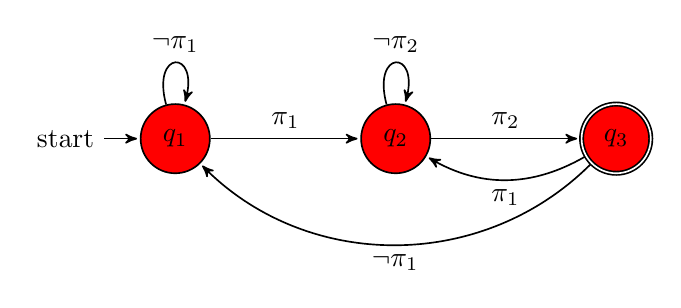
\begin{tikzpicture}[->,>=stealth',shorten >=1pt,auto,node distance=2.8cm,
                    semithick]
  \tikzstyle{every state}=[fill=red,draw=black,text=black]

  \node[initial,state] (A)                    {$q_1$};
  \node[state] (B)                    [right of=A]{$q_2$};
  \node[state,accepting] (C)                    [right of=B]{$q_3$};

  \path (A) edge              node {$\pi_{1}$} (B)
  		(A) edge [loop above] node {$\neg \pi_1$} (A)
  		(B) edge [loop above] node {$\neg \pi_2$} (B)
  		(B) edge              node {$\pi_{2}$} (C)
  		(C) edge [bend left=45] node {$\neg \pi_1$} (A)
  		(C) edge  [bend left] node {$\pi_{1}$} (B);
%  		(D) edge [bend right] node {$\neg \pi_1$} (A)
 % 		(D) edge [bend left] node {$\pi_1$} (B);
\end{tikzpicture}
\caption{B\"uchi Automaton for $\smallsquare(\diamond \pi_1 \land \diamond \pi_2 )$ 1}
\label{fig:gasBuchiRec}
\end{figure}
Note: Again, the actual automaton generated has much more edges. %For example, there is an edge from $q_4$ to $q_2$ which is labelled $\pi_1 \&\& \pi_2$. It is impossible for us to make this transition because $\pi_i$ for all $i$ is a region in our partition. This is because the requirements of our partition are chosen specially to guarantee that we are never in two regions at once. Thus they are excluded in the interest of the reader. 
In this automation, $d(q_1)=2$, $d(q_2)=1$, and $d(q_3)=0$. So, to get from $q_{1}' = \langle \pi_2, q_1 \rangle \in Q_0'$, we have to first get down to level 2. Given the B\"{u}chi automaton \ref{fig:gasBuchiRec} the only way to do this is to go to region $\pi_1$.  In this case the same statement holds for $\pi_2$. It follows that the prefix with the least cost is a concatenation of the shortest paths down from each level (first to $\pi_1$, etc).


This path however is in general not truly optimal. It is because the B\"{u}chi automaton given in figure \ref{fig:gasBuchiRec} not a tight B\"{u}chi automaton. A B\"{u}chi automaton is tight if it accepts the shortest lasso (prefix and suffix). The loss of optimality is due to the fact that the algorithm in \cite{gastin01} simplifies the B\"{u}chi automaton. This is usually a good thing because it leads to a lower computational complexity in most applications. We take a look at a different automaton corresponding to the formula $\smallsquare(\diamond \pi_1 \land \diamond \pi_2)$, shown in figure \ref{fig:otherBuchiRec}. 

\begin{figure}
\centering
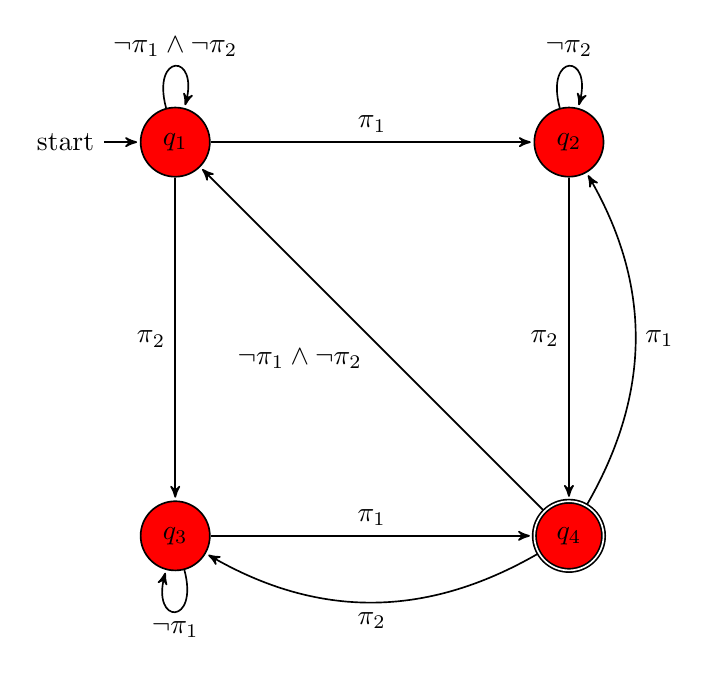
\begin{tikzpicture}[->,>=stealth',shorten >=1pt,auto,node distance=5cm,
                    semithick]
  \tikzstyle{every state}=[fill=red,draw=black,text=black]

  \node[initial,state] (A)                    {$q_1$};
  \node[state]         (B) [ right of=A] {$q_2$};  
  \node[state] 		   (C)  [below of=A]  {$q_3$};
  \node[state,accepting]       (D) [ right of=C] {$q_4$};

  \path (A) edge         node {$\pi_{1}$}   (B)
        (B) edge       node [swap] {$\pi_{2}$}    (D)
        (A) edge       node [swap] {$\pi_{2}$}  (C)
        (C) edge     node {$\pi_{1}$}       (D)
        (A) edge [loop above] node {$\neg \pi_1 \wedge \neg \pi_2$} (A)
        (B) edge [loop above] node {$\neg \pi_2$} (B)
        (C) edge [loop below] node {$\neg \pi_1$} (C)
        (D) edge [bend left] node {$\pi_2$} (C)
        (D) edge [bend right] node [swap] {$\pi_1$} (B)
        (D) edge node{$\neg \pi_1 \wedge \neg \pi_2$} (A);
\end{tikzpicture}
\caption{B\"uchi Automaton for $\smallsquare(\diamond \pi_1 \land \diamond \pi_2)$ 2}
\label{fig:otherBuchiRec}
\end{figure}

In this automaton, $d(q_1) = 2$, $d(q_2) = d(q_3) = 1$, and $d(q_4)= 0$. So, we are starting at the same level, however this time we have to choices of ways to get down to level 2; we can go to $\pi_1$ or $\pi_2$. Being able to choose is good in the sense that we can now find the truly optimal path, and bad in the sense that the extra state in the $B\"{u}chi$ automaton increased the size of the product automaton by 33\% (hence increasing the time it takes to search the automaton). This very well illustrates the trade off between the search time and cost of the resulting path. We propose that this is a good way to think about the greedy algorithm. It is a trade off: sometimes it will not find the optimal run, though it will be faster. 

\subsection{Suffix}
The second aspect of this problem that we wish to look at is fact that it does not have a trivial suffix. In the other examples we have looked at, the suffix of the calculated path was a single state; that is, the formula could be satisfied by staying in one state forever. In this example, $\pi_1,$ $\pi_2$, and $\pi_3$ must all be visited infinitely often, and thus these states must be in the suffix. 

The applicability of the greedy algorithm to find the suffix has to be considered. For any path, R, to be accepting, $\Inf(R) \cap \F$ must not be empty. We are specifically looking for runs of the form 

\begin{align*}
R &= \langle R_{pre}, R_{suf} \rangle = q_0' q_1' \dots {\color{red} q_f'} [q_{f+1}' \dots q_n' {\color{red} q_f'}]^\omega \\
\end{align*}

%\begin{align*}
%R &= \langle R_{pre}, R_{suf} \rangle = q_0 q_1 \dots q_f [q_f q_{f+1} \dots q_n]^\omega
%\end{align*}     
where ${\color{red} q_f'} \in \F'$. Thus when calculating the suffix we must find the path from an accepting state back to the \textit{same} accepting state. We cannot not just look for any accepting state as we do in the prefix calculation. The idea of decreasing levels only looks for an accepting state, not a specific accepting state. Thus we have to do a Dijkstra search and if there is a path back to the accepting state it will find it. The greedy algorithm does have the benefit that it only has to find the shortest path back to one accepting state, not all of them.
%We notice how in figure \ref{fig:gasBuchiRec} there is only one arrow to the accepting state, labelled $\pi_5$. This implies that the only way to get down to level 0 is to go to $\pi_5$, and thus go to the accepting state $\langle \pi_5, q_3 \rangle$. There is no self loop on $q_3$, so we leave $q_3$ immediately. This implies that the only reachable accepting state is $\langle \pi_5, q_3 \rangle$. So because there is only one accepting state, our algorithm will find this state again, and thus is appropriate for finding the suffix. 

%In \ref{fig:otherBuchiRec} on the other hand, there are two arrows going to the accepting state and there is no self loop. This implies that there are two reachable accepting states i.e.\ $\langle \pi_3, q_4 \rangle$ and $\langle \pi_5, q_4 \rangle$. This poses a problem to our algorithm that is only guaranteed to reach an accepting state. We thus propose using Dijkstra's search algorithm to find the path from the accepting node back to itself.   

\subsection{Simulation}





We have shown previously that given the B\"{u}chi automaton by \cite{ltlbuchiwebsite}, the prefix with the least cost is a concatenation of the shortest paths down from each each level (first to $\pi_1$, etc.). The greedy algorithm goes to $\pi_1$ where it can get down a level and then starts a new Dijkstra search. The greedy algorithm does a Dijkstra search at each level so it will return this path as the prefix. The accepted algorithm will also return this prefix. 

The algorithms produced the same path. The accepted algorithm did this in \\


\begin{minipage}{\textwidth}
\begingroup
\fontsize{9pt}{12pt}\selectfont
\begin{lstlisting}
Accepted Algorithm
==================
accepted_plan done within 16.17s: precost 62.00, sufcost 60.00
...
full construction and synthesis done within 16.35s 
\end{lstlisting}
\endgroup
\end{minipage} \\ \\


while the greedy algorithm did it in \\


\begin{minipage}{\textwidth}
\begingroup
\fontsize{9pt}{12pt}\selectfont
\begin{lstlisting}
Greedy Algorithm
================
greedy_plan done within 0.04s: precost 62.00, sufcost 60.00
...
full construction and synthesis done within 0.21s 
\end{lstlisting}
\endgroup
\end{minipage} \\ \\


As we can see, this is the greatest difference in times out of all the examples so far. But why? This is the first example when the suffix is not trivial. In the greedy algorithm, again we search 326+266+587 = 1179 nodes to find the first accepting node. It then does a Dijkstra search to find the shortest path back to this accepting node. This search searches 1875 nodes, resulting in a total search of 3054 nodes. The accepted algorithm does a search of 1875 to find the accepting nodes, and then a search from every accepting node back to itself. These searches are not trivial any more, so each of these searches look through 1875 nodes. Since there are 625 accepting nodes, this results in searching 1173750 nodes. This is where the difference comes from. 

\newpage
\FloatBarrier
\section{More Complex Formulas}
The formulas in the previous section are common formulas, however they are fairly simple and only cover a small subset of the infinite amount of possible formulas that can be formed by temporal logics. The benefit of using temporal logics is that a wide variety of behaviours can be expressed, including propositions about the robot \textit{and} about the workspace. Up to now, we have not looked at any formulas that include atomic propositions about potential tasks. We will show through examples that the same ideas presented in the previous chapter still hold true for this complex tasks, and show the speed up we get by using our algorithm compared to the accepted algorithm. 

\subsection{Example 1}
We look at the example from \cite{guo15} which says "eventually pick up the red ball. Once it is done, move to one basket and drop it. At last come back to room one and stay there". This task can be written as the LTL formula $\varphi = \diamond (\text{pickrball} \wedge \diamond \text{droprball}) \wedge \diamond \smallsquare r1$. The B\"uchi automaton corresponding to this formula as translated by \cite{gastin01} is shown in figure \ref{fig:buchiEx1}, with pick being short for pickrball and drop being short for droprball.

\begin{figure*}[!htb]
\centering
\includegraphics[scale=0.4]{buchiEx1_1}
\caption{B\"uchi Automaton Corresponding to $\varphi = \diamond (\text{pickrball} \wedge \diamond \text{droprball}) \wedge \diamond \smallsquare r1$}
\label{fig:buchiEx1}
\end{figure*} 

As we can see, there are many edges in this automaton and edges that have \&\& in the label. These paths can only be taken if we satisfy both of the propositions at the same time. However, because in our example the propositions do not overlap (the ball is not in the same room as the basket, and the neither the ball or basket is located in room 1) these edge are impossible to take. Therefore we remove these edges from the automaton. We then have a much simpler automaton that is shown in figure \ref{fig:ex1SimplifiedBuchi}

\begin{figure}
\centering
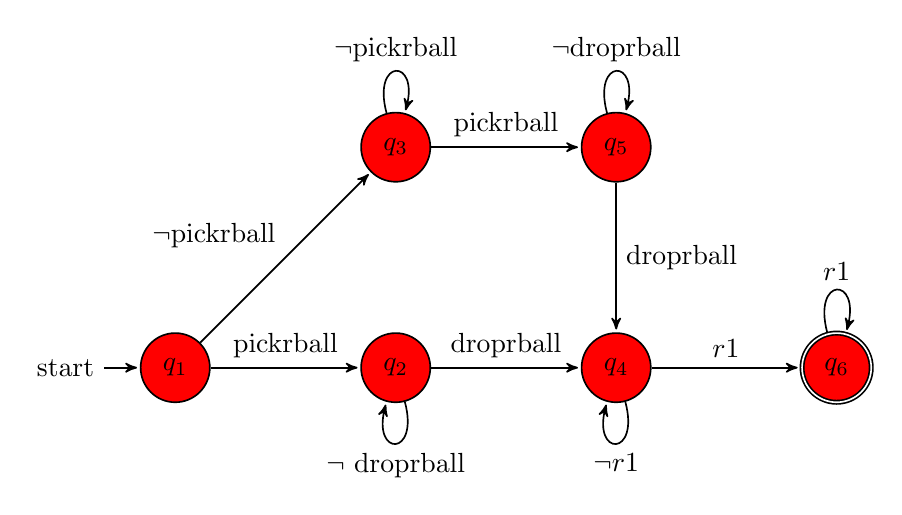
\begin{tikzpicture}[->,>=stealth',shorten >=1pt,auto,node distance=2.8cm,
                    semithick]
  \tikzstyle{every state}=[fill=red,draw=black,text=black]

  \node[initial,state] (A)                    {$q_1$};
  \node[state] (B)                    [right of=A]{$q_2$};
  \node[state] (C)                    [right of=B]{$q_4$};
  \node[state] (E)                    [above of=B]{$q_3$};
  \node[state] (F)                    [above of=C]{$q_5$};
  \node[state,accepting]         (D) [right of=C] {$q_6$};

  \path (A) edge              node {pickrball} (B)
  		%(A) edge [loop above] node {$\neg \pi_1$} (A)
  		(B) edge [loop below] node {$\neg$ droprball} (B)
  		(B) edge              node {droprball} (C)
  		(A) edge              node {$\neg$pickrball} (E)
  		(E) edge              node {pickrball} (F)
  		(F) edge              node {droprball} (C)
  		(C) edge [loop below] node {$\neg r1$} (C)
  		(C) edge              node {$r1$} (D)
  		(E) edge [loop above] node {$\neg$pickrball} (E)
  		(F) edge [loop above] node {$\neg$droprball} (F)
  		(D) edge [loop above] node {$r1$} (D);
\end{tikzpicture}
\caption{Simplified B\"uchi Automaton for $\varphi = \diamond (\text{pickrball} \wedge \diamond \text{droprball}) \wedge \diamond \smallsquare r1$ 1}
\label{fig:ex1SimplifiedBuchi}
\end{figure} 

In this automaton, we can see that $d(q_1)=3$, $d(q_2)=2$, $d(q_3)=3$, $d(q_4)=1$, $d(q_5)=2$, $d(q_6)=0$. For the first time, we have a node that connects to the initial node which is on the same level as the initial node. Examining our algorithm, we see that we will not start a new Dijkstra search until we find a node which is a level bellow our current level. Therefore we will not start a new search until we find a node in the product automaton with projection onto $q_2$ or $q_5$.

We can also see that from the illustration of the workspace, that the ball (rball) is not located next to the initial node, so the first proposition must be $\neg$pickrball. Examining the automaton in figure \ref{fig:ex1SimplifiedBuchi} we see we are guaranteed to take a path through nodes with projection $q_3$ and that we will never go to a node with the projection $q_2$. Therefore we are in the same situation as for sequencing i.e.\ there is only one sequence of actions that will satisfy the formula, implying that our algorithm will find the same path as the accepted algorithm, just faster. 

\begin{figure}[!htb]
\centering
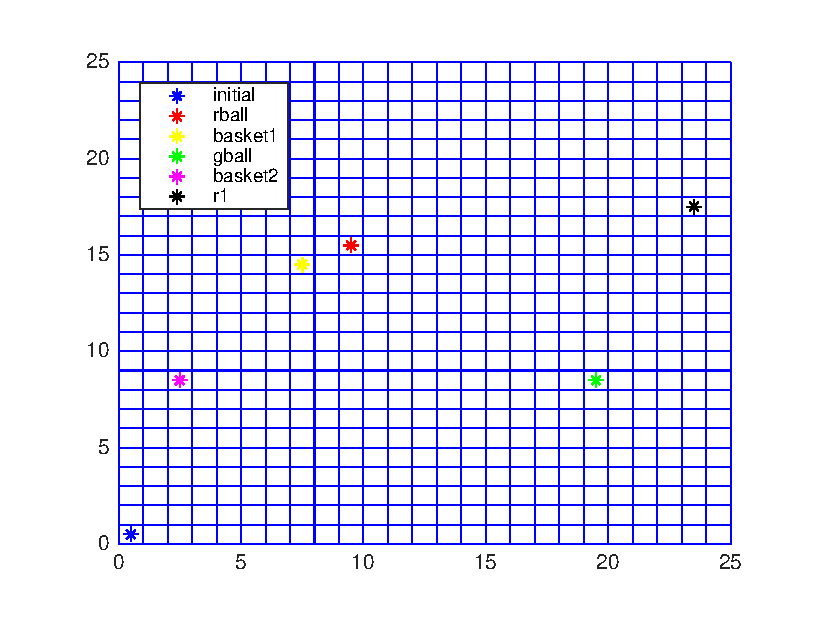
\includegraphics[scale=1]{workspace2.eps}
\label{fig:workspace2}
\caption{Workspace 2}
\end{figure}

We see that this is true in the output of the algorithms. Both give the same sequence of states and actions
\begin{lstlisting}
------------------------------
the prefix of plan **states**:
[((0, 0, 1), 'None'), ((0, 1, 1), 'None'), ((0, 2, 1), 'None'), ((1, 2, 1), 'None'), ((1, 3, 1), 'None'), ((2, 3, 1), 'None'), ((2, 4, 1), 'None'), ((3, 4, 1), 'None'), ((4, 4, 1), 'None'), ((4, 5, 1), 'None'), ((5, 5, 1), 'None'), ((5, 6, 1), 'None'), ((5, 7, 1), 'None'), ((6, 7, 1), 'None'), ((6, 8, 1), 'None'), ((7, 8, 1), 'None'), ((8, 8, 1), 'None'), ((8, 9, 1), 'None'), ((9, 9, 1), 'None'), ((9, 10, 1), 'None'), ((9, 11, 1), 'None'), ((9, 12, 1), 'None'), ((9, 13, 1), 'None'), ((9, 14, 1), 'None'), ((9, 15, 1), 'None'), ((9, 15, 1), 'pickrball'), ((9, 14, 1), 'None'), ((8, 14, 1), 'None'), ((7, 14, 1), 'None'), ((7, 14, 1), 'droprball'), ((7, 15, 1), 'None'), ((7, 16, 1), 'None'), ((7, 17, 1), 'None'), ((8, 17, 1), 'None'), ((9, 17, 1), 'None'), ((10, 17, 1), 'None'), ((11, 17, 1), 'None'), ((12, 17, 1), 'None'), ((13, 17, 1), 'None'), ((14, 17, 1), 'None'), ((15, 17, 1), 'None'), ((16, 17, 1), 'None'), ((17, 17, 1), 'None'), ((18, 17, 1), 'None'), ((19, 17, 1), 'None'), ((20, 17, 1), 'None'), ((21, 17, 1), 'None'), ((22, 17, 1), 'None'), ((23, 17, 1), 'None'), ((23, 17, 1), 'None')]
the suffix of plan **states**:
[((23, 17, 1), 'None'), ((23, 17, 1), 'None')]
------------------------------
the prefix of plan **actions**:
[(0, 0, 1), (0, 1, 1), (0, 2, 1), (1, 2, 1), (1, 3, 1), (2, 3, 1), (2, 4, 1), (3, 4, 1), (4, 4, 1), (4, 5, 1), (5, 5, 1), (5, 6, 1), (5, 7, 1), (6, 7, 1), (6, 8, 1), (7, 8, 1), (8, 8, 1), (8, 9, 1), (9, 9, 1), (9, 10, 1), (9, 11, 1), (9, 12, 1), (9, 13, 1), (9, 14, 1), (9, 15, 1), 'pickrball', (9, 14, 1), (8, 14, 1), (7, 14, 1), 'droprball', (7, 15, 1), (7, 16, 1), (7, 17, 1), (8, 17, 1), (9, 17, 1), (10, 17, 1), (11, 17, 1), (12, 17, 1), (13, 17, 1), (14, 17, 1), (15, 17, 1), (16, 17, 1), (17, 17, 1), (18, 17, 1), (19, 17, 1), (20, 17, 1), (21, 17, 1), (22, 17, 1), (23, 17, 1), 'None', 'None']
the suffix of plan **actions**:
['None', 'None']
\end{lstlisting}

Our algorithm gives 
\begin{lstlisting}
Our Algorithm
==================
new_algorithm_plan done within 0.03s: precost 66.00, sufcost 0.00
\end{lstlisting}
while the accepted algorithm gives 

\begin{lstlisting}
Accepted Algorithm
==================
Dijkstra_plan_networkX done within 0.05s: precost 66.00, sufcost 0.00
\end{lstlisting}

We note here pickrball and droprball are potential tasks i.e.\ they belong in $AP_p$. They are incoded in the action model in the P\_MAS\_TG framework. pickrball can only be done if rball is true, and this is only true in the region corresponding to (9,15).  droprball can only be done if basket1 is true, and this is only true in the region corresponding to (7,14) (see figure \ref{fig:workspace2}). We give both of these actions an arbitrary cost of 10. The way P\_MAS\_TG treats actions gives increases the size of the product automaton by three fold. This is because when a predicate is incoded as an action, each state has corresponding states for doing that action in this state. So instead of having a product automaton of size $|\text{FTS}| \times |\text{B\"uchi}| $ we have a size $|\text{FTS}| \times |\text{B\"uchi}| \times |\text{possible actions}|$. The possible actions in this case are \{ "none", "pickrball", "droprball" \}. We said that pickrball was only possible when rball is true and droprball is only possible when basket1 is true. This statement is still valid, the resulting contradictory nodes simply have no edges leading to them so they cannot be reached. 


\subsection{Example 1 Overlapping Regions}
We now look at the same example, except now we have a different workspace. We choose this example to show what happens if the regions of interest are overlapping. Because of the way the code is structured, we are not able to make take transitions with two or more propositions at one time. We show the example if rball is in the same area as the basket. If this is the case, then pickrball and dropbasket could theoretically be done simultaneously. However, this is not possible because of the code. The only possible transitions that we can take that include \&\& have to be a region and a potential task. We leave the transitions satisfying this requirement and remove all others so the algorithm can have a better distances to follow. The automaton is now
\begin{figure}
\centering
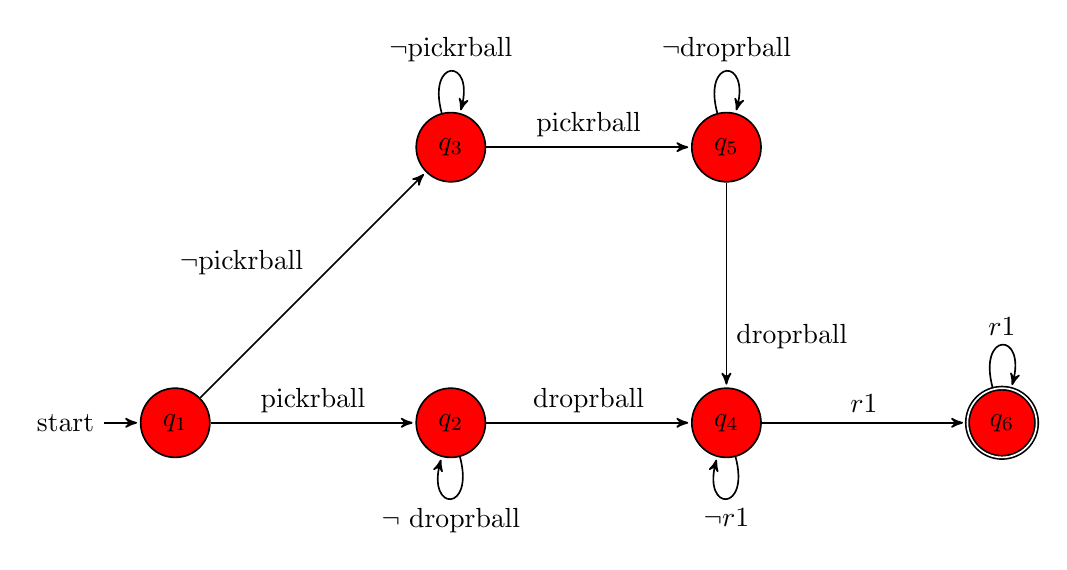
\begin{tikzpicture}[->,>=stealth',shorten >=1pt,auto,node distance=3.5cm,
                    semithick]
  \tikzstyle{every state}=[fill=red,draw=black,text=black]

  \node[initial,state] (A)                    {$q_1$};
  \node[state] (B)                    [right of=A]{$q_2$};
  \node[state] (C)                    [right of=B]{$q_4$};
  \node[state] (E)                    [above of=B]{$q_3$};
  \node[state] (F)                    [above of=C]{$q_5$};
  \node[state,accepting]         (D) [right of=C] {$q_6$};

  \path (A) edge              node {pickrball} (B)
  		%(A) edge   [bend right=90]	 node {rball \&\& basket} (C)
  		%(E) edge		[near start]			node {rball \&\& basket} (C)
  		%(A) edge [loop above] node {$\neg \pi_1$} (A)
  		(B) edge [loop below] node {$\neg$ droprball} (B)
  		(B) edge              node {droprball} (C)
  		(A) edge              node {$\neg$pickrball} (E)
  		(E) edge              node {pickrball} (F)
  		(F) edge        [near end]      node {droprball} (C)
  		(C) edge [loop below] node {$\neg r1$} (C)
  		(C) edge              node {$r1$} (D)
  		(E) edge [loop above] node {$\neg$pickrball} (E)
  		(F) edge [loop above] node {$\neg$droprball} (F)
  		(D) edge [loop above] node {$r1$} (D);
\end{tikzpicture}
\caption{Simplified B\"uchi Automaton Corresponding to $\varphi = \diamond (\text{pickrball} \wedge \diamond \text{droprball}) \wedge \diamond \smallsquare r1$ 2}
\label{fig:ex1OverlapSimplifiedBuchi}
\end{figure} 

In this automaton, we now have $d(q_1)=3$, $d(q_2)=2$, $d(q_3)=3$, $d(q_4)=1$, $d(q_5) = 2$ and $d(q_6)=0$. We see again that rball and basket are not one step away from the initial node, implying that we cannot take the first step pickrball. This means that we can never go to $q_2$, and that there is only one path through the automaton to take. Therefore our algorithm is guaranteed to compute the same path as the accepted algorithm and it will do so in less time.

We look at the results and see that our algorithm indeed calculates the same path in a shorter amount of time than the accepted algorithm.

\begin{lstlisting}
Accepted Algorithm
==================
Dijkstra_plan_networkX done within 0.05s: precost 60.00, sufcost 0.00
------------------------------
the prefix of plan **states**:
[((0, 0, 1), 'None'), ((0, 1, 1), 'None'), ((0, 2, 1), 'None'), ((1, 2, 1), 'None'), ((1, 3, 1), 'None'), ((2, 3, 1), 'None'), ((2, 4, 1), 'None'), ((3, 4, 1), 'None'), ((4, 4, 1), 'None'), ((4, 5, 1), 'None'), ((5, 5, 1), 'None'), ((5, 6, 1), 'None'), ((5, 7, 1), 'None'), ((6, 7, 1), 'None'), ((6, 8, 1), 'None'), ((7, 8, 1), 'None'), ((8, 8, 1), 'None'), ((8, 9, 1), 'None'), ((9, 9, 1), 'None'), ((9, 10, 1), 'None'), ((9, 11, 1), 'None'), ((9, 12, 1), 'None'), ((9, 13, 1), 'None'), ((9, 14, 1), 'None'), ((9, 15, 1), 'None'), ((9, 15, 1), 'pickrball'), ((9, 15, 1), 'droprball'), ((10, 15, 1), 'None'), ((10, 16, 1), 'None'), ((11, 16, 1), 'None'), ((12, 16, 1), 'None'), ((12, 17, 1), 'None'), ((13, 17, 1), 'None'), ((14, 17, 1), 'None'), ((15, 17, 1), 'None'), ((16, 17, 1), 'None'), ((17, 17, 1), 'None'), ((18, 17, 1), 'None'), ((19, 17, 1), 'None'), ((20, 17, 1), 'None'), ((21, 17, 1), 'None'), ((22, 17, 1), 'None'), ((23, 17, 1), 'None'), ((23, 17, 1), 'None')]
the suffix of plan **states**:
[((23, 17, 1), 'None'), ((23, 17, 1), 'None')]
------------------------------
the prefix of plan **actions**:
[(0, 0, 1), (0, 1, 1), (0, 2, 1), (1, 2, 1), (1, 3, 1), (2, 3, 1), (2, 4, 1), (3, 4, 1), (4, 4, 1), (4, 5, 1), (5, 5, 1), (5, 6, 1), (5, 7, 1), (6, 7, 1), (6, 8, 1), (7, 8, 1), (8, 8, 1), (8, 9, 1), (9, 9, 1), (9, 10, 1), (9, 11, 1), (9, 12, 1), (9, 13, 1), (9, 14, 1), (9, 15, 1), 'pickrball', 'droprball', (10, 15, 1), (10, 16, 1), (11, 16, 1), (12, 16, 1), (12, 17, 1), (13, 17, 1), (14, 17, 1), (15, 17, 1), (16, 17, 1), (17, 17, 1), (18, 17, 1), (19, 17, 1), (20, 17, 1), (21, 17, 1), (22, 17, 1), (23, 17, 1), 'None', 'None']
the suffix of plan **actions**:
['None', 'None']
full construction and synthesis done within 1.11s 
\end{lstlisting}
. \\
. \\
.\\
\begin{lstlisting}
==================
new_algorithm_plan done within 0.02s: precost 60.00, sufcost 0.00
------------------------------
the prefix of plan **states**:
[((0, 0, 1), 'None'), ((0, 1, 1), 'None'), ((0, 2, 1), 'None'), ((1, 2, 1), 'None'), ((1, 3, 1), 'None'), ((2, 3, 1), 'None'), ((2, 4, 1), 'None'), ((3, 4, 1), 'None'), ((4, 4, 1), 'None'), ((4, 5, 1), 'None'), ((5, 5, 1), 'None'), ((5, 6, 1), 'None'), ((5, 7, 1), 'None'), ((6, 7, 1), 'None'), ((6, 8, 1), 'None'), ((7, 8, 1), 'None'), ((8, 8, 1), 'None'), ((8, 9, 1), 'None'), ((9, 9, 1), 'None'), ((9, 10, 1), 'None'), ((9, 11, 1), 'None'), ((9, 12, 1), 'None'), ((9, 13, 1), 'None'), ((9, 14, 1), 'None'), ((9, 15, 1), 'None'), ((9, 15, 1), 'pickrball'), ((9, 15, 1), 'droprball'), ((10, 15, 1), 'None'), ((10, 16, 1), 'None'), ((11, 16, 1), 'None'), ((12, 16, 1), 'None'), ((12, 17, 1), 'None'), ((13, 17, 1), 'None'), ((14, 17, 1), 'None'), ((15, 17, 1), 'None'), ((16, 17, 1), 'None'), ((17, 17, 1), 'None'), ((18, 17, 1), 'None'), ((19, 17, 1), 'None'), ((20, 17, 1), 'None'), ((21, 17, 1), 'None'), ((22, 17, 1), 'None'), ((23, 17, 1), 'None'), ((23, 17, 1), 'None')]
the suffix of plan **states**:
[((23, 17, 1), 'None'), ((23, 17, 1), 'None')]
------------------------------
the prefix of plan **actions**:
[(0, 0, 1), (0, 1, 1), (0, 2, 1), (1, 2, 1), (1, 3, 1), (2, 3, 1), (2, 4, 1), (3, 4, 1), (4, 4, 1), (4, 5, 1), (5, 5, 1), (5, 6, 1), (5, 7, 1), (6, 7, 1), (6, 8, 1), (7, 8, 1), (8, 8, 1), (8, 9, 1), (9, 9, 1), (9, 10, 1), (9, 11, 1), (9, 12, 1), (9, 13, 1), (9, 14, 1), (9, 15, 1), 'pickrball', 'droprball', (10, 15, 1), (10, 16, 1), (11, 16, 1), (12, 16, 1), (12, 17, 1), (13, 17, 1), (14, 17, 1), (15, 17, 1), (16, 17, 1), (17, 17, 1), (18, 17, 1), (19, 17, 1), (20, 17, 1), (21, 17, 1), (22, 17, 1), (23, 17, 1), 'None', 'None']
the suffix of plan **actions**:
['None', 'None']
full construction and synthesis done within 1.09s 
\end{lstlisting}



\subsection{Example 2}
We now look at the example taken from \cite{guo15} in which the robot has to pick up and deliver two different balls (rball and gball) to two different baskets, and the robot cannot carry two balls at once. After this is done the robot is to go to r1 and stay there. This task is formalized as $\varphi = \diamond (\text{pickrball} \wedge \diamond (\text{droprball})) \wedge \diamond(\text{pickgball} \wedge \diamond (\text{dropgball})) \wedge \smallsquare (\text{pickrball} \rightarrow \textbf{X}(\neg \text{pickgball} \U \text{droprball})) \wedge \smallsquare (\text{pickgball} \rightarrow \textbf{X} (\neg \text{pickrball} \U \text{dropgball})) \&\& \diamond \smallsquare r1$. This formula formalizes the basket corresponding to rball is in region r2 and the basket corresponding to gball is in r4. The B\"uchi automaton corresponding to this formula is much to large to show. It has 75 states and 797 edges. If the reader is interested, the automaton can be found using the online tool \cite{ltlbuchiwebsite} with the input F(pickrball \&\& F(droprball)) \&\& F(pickgball \&\& F(dropgball)) \&\& G(pickrball -> X(! pickgball U droprball)) \&\& G(pickgball -> X(! pickrball U dropgball)) \&\& F(G(r1)). It is too large for the tool to give a visual representation but it will provide a list of states and edges.  

To analyse the performance of our algorithm on this problem, we are going to break up this problem into the choices that the robot has. The robot has to pick up one of the balls, return it to the corresponding basket, then pick up the second ball and return it to its corresponding basket. Assuming that everything else is done in the optimal way, the only choice that must be made is which ball to pick up first. This is the output, accepted algorithm first:

\begin{lstlisting}
Accepted Algorithm
==================
Dijkstra_plan_networkX done within 0.63s: precost 118.00, sufcost 0.00
------------------------------
the prefix of plan **states**:
[((0, 0, 1), 'None'), ((1, 0, 1), 'None'), ((1, 1, 1), 'None'), ((2, 1, 1), 'None'), ((2, 2, 1), 'None'), ((3, 2, 1), 'None'), ((3, 3, 1), 'None'), ((4, 3, 1), 'None'), ((5, 3, 1), 'None'), ((6, 3, 1), 'None'), ((7, 3, 1), 'None'), ((8, 3, 1), 'None'), ((8, 4, 1), 'None'), ((9, 4, 1), 'None'), ((10, 4, 1), 'None'), ((11, 4, 1), 'None'), ((12, 4, 1), 'None'), ((13, 4, 1), 'None'), ((14, 4, 1), 'None'), ((15, 4, 1), 'None'), ((16, 4, 1), 'None'), ((16, 5, 1), 'None'), ((16, 6, 1), 'None'), ((17, 6, 1), 'None'), ((18, 6, 1), 'None'), ((19, 6, 1), 'None'), ((19, 7, 1), 'None'), ((19, 8, 1), 'None'), ((19, 8, 1), 'pickgball'), ((19, 9, 1), 'None'), ((18, 9, 1), 'None'), ((18, 10, 1), 'None'), ((17, 10, 1), 'None'), ((16, 10, 1), 'None'), ((15, 10, 1), 'None'), ((14, 10, 1), 'None'), ((13, 10, 1), 'None'), ((12, 10, 1), 'None'), ((11, 10, 1), 'None'), ((10, 10, 1), 'None'), ((9, 10, 1), 'None'), ((8, 10, 1), 'None'), ((7, 10, 1), 'None'), ((6, 10, 1), 'None'), ((5, 10, 1), 'None'), ((4, 10, 1), 'None'), ((3, 10, 1), 'None'), ((2, 10, 1), 'None'), ((2, 10, 1), 'dropgball'), ((2, 11, 1), 'None'), ((2, 12, 1), 'None'), ((2, 13, 1), 'None'), ((2, 14, 1), 'None'), ((3, 14, 1), 'None'), ((4, 14, 1), 'None'), ((5, 14, 1), 'None'), ((5, 15, 1), 'None'), ((6, 15, 1), 'None'), ((7, 15, 1), 'None'), ((8, 15, 1), 'None'), ((9, 15, 1), 'None'), ((9, 15, 1), 'pickrball'), ((8, 15, 1), 'None'), ((7, 15, 1), 'None'), ((7, 14, 1), 'None'), ((7, 14, 1), 'droprball'), ((8, 14, 1), 'None'), ((8, 15, 1), 'None'), ((9, 15, 1), 'None'), ((10, 15, 1), 'None'), ((11, 15, 1), 'None'), ((12, 15, 1), 'None'), ((12, 16, 1), 'None'), ((13, 16, 1), 'None'), ((14, 16, 1), 'None'), ((15, 16, 1), 'None'), ((16, 16, 1), 'None'), ((17, 16, 1), 'None'), ((18, 16, 1), 'None'), ((19, 16, 1), 'None'), ((20, 16, 1), 'None'), ((21, 16, 1), 'None'), ((22, 16, 1), 'None'), ((22, 16, 1), 'None')]
the suffix of plan **states**:
[((22, 16, 1), 'None'), ((22, 16, 1), 'None')]
------------------------------
the prefix of plan **actions**:
[(0, 0, 1), (1, 0, 1), (1, 1, 1), (2, 1, 1), (2, 2, 1), (3, 2, 1), (3, 3, 1), (4, 3, 1), (5, 3, 1), (6, 3, 1), (7, 3, 1), (8, 3, 1), (8, 4, 1), (9, 4, 1), (10, 4, 1), (11, 4, 1), (12, 4, 1), (13, 4, 1), (14, 4, 1), (15, 4, 1), (16, 4, 1), (16, 5, 1), (16, 6, 1), (17, 6, 1), (18, 6, 1), (19, 6, 1), (19, 7, 1), (19, 8, 1), 'pickgball', (19, 9, 1), (18, 9, 1), (18, 10, 1), (17, 10, 1), (16, 10, 1), (15, 10, 1), (14, 10, 1), (13, 10, 1), (12, 10, 1), (11, 10, 1), (10, 10, 1), (9, 10, 1), (8, 10, 1), (7, 10, 1), (6, 10, 1), (5, 10, 1), (4, 10, 1), (3, 10, 1), (2, 10, 1), 'dropgball', (2, 11, 1), (2, 12, 1), (2, 13, 1), (2, 14, 1), (3, 14, 1), (4, 14, 1), (5, 14, 1), (5, 15, 1), (6, 15, 1), (7, 15, 1), (8, 15, 1), (9, 15, 1), 'pickrball', (8, 15, 1), (7, 15, 1), (7, 14, 1), 'droprball', (8, 14, 1), (8, 15, 1), (9, 15, 1), (10, 15, 1), (11, 15, 1), (12, 15, 1), (12, 16, 1), (13, 16, 1), (14, 16, 1), (15, 16, 1), (16, 16, 1), (17, 16, 1), (18, 16, 1), (19, 16, 1), (20, 16, 1), (21, 16, 1), (22, 16, 1), 'None', 'None']
the suffix of plan **actions**:
['None', 'None']
full construction and synthesis done within 55.25s 
\end{lstlisting}
and our algorithm
\begin{lstlisting}
==================
new_algorithm_plan done within 0.28s: precost 130.00, sufcost 0.00
------------------------------
the prefix of plan **states**:
[((0, 0, 1), 'None'), ((0, 1, 1), 'None'), ((0, 2, 1), 'None'), ((1, 2, 1), 'None'), ((2, 2, 1), 'None'), ((3, 2, 1), 'None'), ((4, 2, 1), 'None'), ((4, 3, 1), 'None'), ((5, 3, 1), 'None'), ((5, 4, 1), 'None'), ((6, 4, 1), 'None'), ((7, 4, 1), 'None'), ((7, 5, 1), 'None'), ((8, 5, 1), 'None'), ((8, 6, 1), 'None'), ((8, 7, 1), 'None'), ((8, 8, 1), 'None'), ((8, 9, 1), 'None'), ((9, 9, 1), 'None'), ((9, 10, 1), 'None'), ((9, 11, 1), 'None'), ((9, 12, 1), 'None'), ((9, 13, 1), 'None'), ((9, 14, 1), 'None'), ((9, 15, 1), 'None'), ((9, 15, 1), 'pickrball'), ((9, 14, 1), 'None'), ((8, 14, 1), 'None'), ((7, 14, 1), 'None'), ((7, 14, 1), 'droprball'), ((8, 14, 1), 'None'), ((8, 13, 1), 'None'), ((8, 12, 1), 'None'), ((9, 12, 1), 'None'), ((10, 12, 1), 'None'), ((11, 12, 1), 'None'), ((11, 11, 1), 'None'), ((11, 10, 1), 'None'), ((12, 10, 1), 'None'), ((12, 9, 1), 'None'), ((13, 9, 1), 'None'), ((14, 9, 1), 'None'), ((15, 9, 1), 'None'), ((15, 8, 1), 'None'), ((16, 8, 1), 'None'), ((17, 8, 1), 'None'), ((18, 8, 1), 'None'), ((19, 8, 1), 'None'), ((19, 8, 1), 'pickgball'), ((18, 8, 1), 'None'), ((18, 9, 1), 'None'), ((18, 10, 1), 'None'), ((17, 10, 1), 'None'), ((16, 10, 1), 'None'), ((15, 10, 1), 'None'), ((14, 10, 1), 'None'), ((13, 10, 1), 'None'), ((12, 10, 1), 'None'), ((11, 10, 1), 'None'), ((10, 10, 1), 'None'), ((9, 10, 1), 'None'), ((8, 10, 1), 'None'), ((7, 10, 1), 'None'), ((6, 10, 1), 'None'), ((5, 10, 1), 'None'), ((4, 10, 1), 'None'), ((3, 10, 1), 'None'), ((2, 10, 1), 'None'), ((2, 10, 1), 'dropgball'), ((2, 11, 1), 'None'), ((2, 12, 1), 'None'), ((2, 13, 1), 'None'), ((3, 13, 1), 'None'), ((3, 14, 1), 'None'), ((4, 14, 1), 'None'), ((4, 15, 1), 'None'), ((4, 16, 1), 'None'), ((5, 16, 1), 'None'), ((6, 16, 1), 'None'), ((7, 16, 1), 'None'), ((8, 16, 1), 'None'), ((9, 16, 1), 'None'), ((10, 16, 1), 'None'), ((11, 16, 1), 'None'), ((12, 16, 1), 'None'), ((13, 16, 1), 'None'), ((14, 16, 1), 'None'), ((15, 16, 1), 'None'), ((16, 16, 1), 'None'), ((17, 16, 1), 'None'), ((18, 16, 1), 'None'), ((19, 16, 1), 'None'), ((20, 16, 1), 'None'), ((21, 16, 1), 'None'), ((22, 16, 1), 'None'), ((22, 16, 1), 'None')]
the suffix of plan **states**:
[((22, 16, 1), 'None'), ((22, 16, 1), 'None')]
------------------------------
the prefix of plan **actions**:
[(0, 0, 1), (0, 1, 1), (0, 2, 1), (1, 2, 1), (2, 2, 1), (3, 2, 1), (4, 2, 1), (4, 3, 1), (5, 3, 1), (5, 4, 1), (6, 4, 1), (7, 4, 1), (7, 5, 1), (8, 5, 1), (8, 6, 1), (8, 7, 1), (8, 8, 1), (8, 9, 1), (9, 9, 1), (9, 10, 1), (9, 11, 1), (9, 12, 1), (9, 13, 1), (9, 14, 1), (9, 15, 1), 'pickrball', (9, 14, 1), (8, 14, 1), (7, 14, 1), 'droprball', (8, 14, 1), (8, 13, 1), (8, 12, 1), (9, 12, 1), (10, 12, 1), (11, 12, 1), (11, 11, 1), (11, 10, 1), (12, 10, 1), (12, 9, 1), (13, 9, 1), (14, 9, 1), (15, 9, 1), (15, 8, 1), (16, 8, 1), (17, 8, 1), (18, 8, 1), (19, 8, 1), 'pickgball', (18, 8, 1), (18, 9, 1), (18, 10, 1), (17, 10, 1), (16, 10, 1), (15, 10, 1), (14, 10, 1), (13, 10, 1), (12, 10, 1), (11, 10, 1), (10, 10, 1), (9, 10, 1), (8, 10, 1), (7, 10, 1), (6, 10, 1), (5, 10, 1), (4, 10, 1), (3, 10, 1), (2, 10, 1), 'dropgball', (2, 11, 1), (2, 12, 1), (2, 13, 1), (3, 13, 1), (3, 14, 1), (4, 14, 1), (4, 15, 1), (4, 16, 1), (5, 16, 1), (6, 16, 1), (7, 16, 1), (8, 16, 1), (9, 16, 1), (10, 16, 1), (11, 16, 1), (12, 16, 1), (13, 16, 1), (14, 16, 1), (15, 16, 1), (16, 16, 1), (17, 16, 1), (18, 16, 1), (19, 16, 1), (20, 16, 1), (21, 16, 1), (22, 16, 1), 'None', 'None']
the suffix of plan **actions**:
['None', 'None']
full construction and synthesis done within 57.55s 
\end{lstlisting}
as we can see, our algorithm picks the closest ball (rball) first even though it is not optimal overall. The added cost is relatively small though, only 12. However, it is possible that the difference could be much larger. In an analysis of speed, our algorithm does the search faster, In about half the time. In either case, the actual search takes around or less than a hundredth of the total time.

\subsection{Example 2 Modified}
We now look at a modified version of example two. Say the robot has to pick up and deliver two different balls (rball and gball) to two different baskets, and the robot cannot carry two balls at once and that is it. There is no need to go to r1, or do anything after the balls are returned to their respective baskets. This task is formalized as $\varphi = \diamond (\text{pickrball} \wedge \diamond (\text{droprball})) \wedge \diamond(\text{pickgball} \wedge \diamond (\text{dropgball})) \wedge \smallsquare (\text{pickrball} \rightarrow \textbf{X}(\neg \text{pickgball} \U \text{droprball})) \wedge \smallsquare (\text{pickgball} \rightarrow \\ \textbf{X} (\neg \text{pickrball} \U \text{dropgball}))$. This version seems easier than original example. The B\"uchi automaton for this formula would seem to agree; it is smaller, with 38 nodes and 308 edges. However, here is the out put from both algorithms:

\begin{lstlisting}
Accepted Algorithm
==================
Dijkstra_plan_networkX done within 926.40s: precost 101.00, sufcost 0.00
------------------------------
the prefix of plan **states**:
[((0, 0, 1), 'None'), ((1, 0, 1), 'None'), ((1, 1, 1), 'None'), ((1, 2, 1), 'None'), ((2, 2, 1), 'None'), ((2, 3, 1), 'None'), ((3, 3, 1), 'None'), ((4, 3, 1), 'None'), ((5, 3, 1), 'None'), ((6, 3, 1), 'None'), ((7, 3, 1), 'None'), ((7, 4, 1), 'None'), ((8, 4, 1), 'None'), ((9, 4, 1), 'None'), ((10, 4, 1), 'None'), ((11, 4, 1), 'None'), ((12, 4, 1), 'None'), ((12, 5, 1), 'None'), ((12, 6, 1), 'None'), ((13, 6, 1), 'None'), ((13, 7, 1), 'None'), ((13, 8, 1), 'None'), ((14, 8, 1), 'None'), ((15, 8, 1), 'None'), ((16, 8, 1), 'None'), ((17, 8, 1), 'None'), ((18, 8, 1), 'None'), ((19, 8, 1), 'None'), ((19, 8, 1), 'pickgball'), ((18, 8, 1), 'None'), ((17, 8, 1), 'None'), ((17, 9, 1), 'None'), ((17, 10, 1), 'None'), ((16, 10, 1), 'None'), ((15, 10, 1), 'None'), ((14, 10, 1), 'None'), ((13, 10, 1), 'None'), ((12, 10, 1), 'None'), ((11, 10, 1), 'None'), ((10, 10, 1), 'None'), ((9, 10, 1), 'None'), ((8, 10, 1), 'None'), ((7, 10, 1), 'None'), ((6, 10, 1), 'None'), ((5, 10, 1), 'None'), ((4, 10, 1), 'None'), ((3, 10, 1), 'None'), ((2, 10, 1), 'None'), ((2, 10, 1), 'dropgball'), ((2, 11, 1), 'None'), ((2, 12, 1), 'None'), ((2, 13, 1), 'None'), ((3, 13, 1), 'None'), ((4, 13, 1), 'None'), ((5, 13, 1), 'None'), ((5, 14, 1), 'None'), ((6, 14, 1), 'None'), ((6, 15, 1), 'None'), ((7, 15, 1), 'None'), ((8, 15, 1), 'None'), ((9, 15, 1), 'None'), ((9, 15, 1), 'pickrball'), ((9, 14, 1), 'None'), ((8, 14, 1), 'None'), ((7, 14, 1), 'None'), ((7, 14, 1), 'droprball'), ((7, 14, 1), 'None')]
the suffix of plan **states**:
[((7, 14, 1), 'None'), ((7, 14, 1), 'None')]
------------------------------
the prefix of plan **actions**:
[(0, 0, 1), (1, 0, 1), (1, 1, 1), (1, 2, 1), (2, 2, 1), (2, 3, 1), (3, 3, 1), (4, 3, 1), (5, 3, 1), (6, 3, 1), (7, 3, 1), (7, 4, 1), (8, 4, 1), (9, 4, 1), (10, 4, 1), (11, 4, 1), (12, 4, 1), (12, 5, 1), (12, 6, 1), (13, 6, 1), (13, 7, 1), (13, 8, 1), (14, 8, 1), (15, 8, 1), (16, 8, 1), (17, 8, 1), (18, 8, 1), (19, 8, 1), 'pickgball', (18, 8, 1), (17, 8, 1), (17, 9, 1), (17, 10, 1), (16, 10, 1), (15, 10, 1), (14, 10, 1), (13, 10, 1), (12, 10, 1), (11, 10, 1), (10, 10, 1), (9, 10, 1), (8, 10, 1), (7, 10, 1), (6, 10, 1), (5, 10, 1), (4, 10, 1), (3, 10, 1), (2, 10, 1), 'dropgball', (2, 11, 1), (2, 12, 1), (2, 13, 1), (3, 13, 1), (4, 13, 1), (5, 13, 1), (5, 14, 1), (6, 14, 1), (6, 15, 1), (7, 15, 1), (8, 15, 1), (9, 15, 1), 'pickrball', (9, 14, 1), (8, 14, 1), (7, 14, 1), 'droprball', 'None', 'None']
the suffix of plan **actions**:
['None', 'None']
full construction and synthesis done within 950.95s 
\end{lstlisting}
and from our algorithm
\begin{lstlisting}
Our Algorithm
==================
new_algorithm_plan done within 0.30s: precost 104.00, sufcost 0.00
------------------------------
the prefix of plan **states**:
[((0, 0, 1), 'None'), ((1, 0, 1), 'None'), ((1, 1, 1), 'None'), ((2, 1, 1), 'None'), ((2, 2, 1), 'None'), ((2, 3, 1), 'None'), ((3, 3, 1), 'None'), ((4, 3, 1), 'None'), ((5, 3, 1), 'None'), ((5, 4, 1), 'None'), ((6, 4, 1), 'None'), ((6, 5, 1), 'None'), ((7, 5, 1), 'None'), ((7, 6, 1), 'None'), ((7, 7, 1), 'None'), ((8, 7, 1), 'None'), ((9, 7, 1), 'None'), ((9, 8, 1), 'None'), ((9, 9, 1), 'None'), ((9, 10, 1), 'None'), ((9, 11, 1), 'None'), ((9, 12, 1), 'None'), ((9, 13, 1), 'None'), ((9, 14, 1), 'None'), ((9, 15, 1), 'None'), ((9, 15, 1), 'pickrball'), ((9, 14, 1), 'None'), ((8, 14, 1), 'None'), ((7, 14, 1), 'None'), ((7, 14, 1), 'droprball'), ((7, 13, 1), 'None'), ((8, 13, 1), 'None'), ((8, 12, 1), 'None'), ((8, 11, 1), 'None'), ((9, 11, 1), 'None'), ((9, 10, 1), 'None'), ((9, 9, 1), 'None'), ((9, 8, 1), 'None'), ((10, 8, 1), 'None'), ((11, 8, 1), 'None'), ((12, 8, 1), 'None'), ((13, 8, 1), 'None'), ((14, 8, 1), 'None'), ((15, 8, 1), 'None'), ((16, 8, 1), 'None'), ((17, 8, 1), 'None'), ((18, 8, 1), 'None'), ((19, 8, 1), 'None'), ((19, 8, 1), 'pickgball'), ((18, 8, 1), 'None'), ((17, 8, 1), 'None'), ((17, 9, 1), 'None'), ((16, 9, 1), 'None'), ((16, 10, 1), 'None'), ((15, 10, 1), 'None'), ((14, 10, 1), 'None'), ((13, 10, 1), 'None'), ((12, 10, 1), 'None'), ((11, 10, 1), 'None'), ((10, 10, 1), 'None'), ((9, 10, 1), 'None'), ((8, 10, 1), 'None'), ((7, 10, 1), 'None'), ((6, 10, 1), 'None'), ((5, 10, 1), 'None'), ((4, 10, 1), 'None'), ((3, 10, 1), 'None'), ((2, 10, 1), 'None'), ((2, 10, 1), 'dropgball'), ((2, 10, 1), 'None')]
the suffix of plan **states**:
[((2, 10, 1), 'None'), ((2, 10, 1), 'None')]
------------------------------
the prefix of plan **actions**:
[(0, 0, 1), (1, 0, 1), (1, 1, 1), (2, 1, 1), (2, 2, 1), (2, 3, 1), (3, 3, 1), (4, 3, 1), (5, 3, 1), (5, 4, 1), (6, 4, 1), (6, 5, 1), (7, 5, 1), (7, 6, 1), (7, 7, 1), (8, 7, 1), (9, 7, 1), (9, 8, 1), (9, 9, 1), (9, 10, 1), (9, 11, 1), (9, 12, 1), (9, 13, 1), (9, 14, 1), (9, 15, 1), 'pickrball', (9, 14, 1), (8, 14, 1), (7, 14, 1), 'droprball', (7, 13, 1), (8, 13, 1), (8, 12, 1), (8, 11, 1), (9, 11, 1), (9, 10, 1), (9, 9, 1), (9, 8, 1), (10, 8, 1), (11, 8, 1), (12, 8, 1), (13, 8, 1), (14, 8, 1), (15, 8, 1), (16, 8, 1), (17, 8, 1), (18, 8, 1), (19, 8, 1), 'pickgball', (18, 8, 1), (17, 8, 1), (17, 9, 1), (16, 9, 1), (16, 10, 1), (15, 10, 1), (14, 10, 1), (13, 10, 1), (12, 10, 1), (11, 10, 1), (10, 10, 1), (9, 10, 1), (8, 10, 1), (7, 10, 1), (6, 10, 1), (5, 10, 1), (4, 10, 1), (3, 10, 1), (2, 10, 1), 'dropgball', 'None', 'None']
the suffix of plan **actions**:
['None', 'None']
full construction and synthesis done within 21.60s
\end{lstlisting} 

This is by far the largest difference in computation times that we have seen thus far! We will show how this difference is caused by the searches from accepting nodes back to themselves.

As before, we have $|\text{product automaton}| =|\text{FTS}| \times |\text{B\"uchi}| \times |\text{possible actions}|$. The FTS still has 625 nodes, this buchi automaton has 38 nodes, and there are 5 possible actions ("none", "pickrball", "droprball", "pickgball", "dropgball"). This makes for a product automaton of 118750. There are 4 accepting states in the B\"uchi automaton. This gives us 12500 accepting nodes in the product automaton. The accepted algorithm calculates a path back from each accepting node back to itself. This calculation is relatively quick if the accepting node can transition back to itself; however, the cost is much longer if it doesn't. It turns out in this example only 629 of the accepting nodes have a self loop, while 11871 do not. It may seem like the accepting nodes should all be able to transfer back to themselves, but they cannot because of the accepting nodes in the B\"uchi automaton. 

Each accepting node in the B\"uchi automaton has a self loop however, the labels of the self loop can make many of these transitions impossible. The four self loop labels for the four accepting nodes of the B\"uchi automaton are (droprball \&\& dropgball), (!pickrball \&\& dropgball), (!pickrball \&\& !pickgball), and (droprball \&\& !pickgball). Thus the only possible self loop is (!pickrball \&\& !pickgball). All other accepting states must look for another path back to themselves, which results in the incredible increase in time. This is likely the largest danger and downside of using the accepted algorithm. The number of accepting states grows with the size of the FTS, the B\"uchi automaton, and the number of possible actions. Then we have to do a search for each of these accepting nodes.  



\subsection{Other Examples}
As we have seen, due to the complexity of the B\"uchi automata it can be very hard to analyse the performance of our algorithm compared to the accepted algorithm with respect to cost for more complex formulas. We therefore provide the results of runs for various formulas in table \ref{table}. We use formulas from the table in \cite{somenzi00} to try to show a comprehensive experimentation. The formulas are run on the workspace in figure \ref{fig:workspace2}. 

\begin{landscape}
\begin{table}[]
\centering
\small
\begin{tabular}{|c|c|c|c|c|}
\hline
Formula & \makecell{Accepted Cost \\ prefix, suffix} & Accepted Time & \makecell{Our Cost \\ prefix, suffix} & Our Time \\ \hline
     '(!r223 U r445) || (!r268 U r435)'  &         27 ,0     &      0.04         &      27,0   &     0.01     \\ \hline
      '!r62 U(!r266 U r422)'  &         38.00 ,0     &       0.05        &     38,0     &     0.02     \\ \hline
       '[]<> r0 -> []<> r317' &         1,0      &       5.06        &    1,0      &    0.00     \\ \hline
       '[]<> r0 <-> []<> r317'  & 1,0		&		10.70		& 1,0 	&  0.00 \\ \hline 
      '!(<><> r498 <-> r541)' &	42.00	&	0.03	&	42.00	&	0.02	\\		\hline
      '!([]<> r3 -> []<>r591)' &	 3.00, 0	&	5.06 	&	3.00, 0 	&	0.00	\\		\hline
      '!([]<> r3 <-> []<>r591)' &	 3.00, 0	&	10.31	&	39, 0	&	0.01	\\		\hline
      '!r532 R (!r432 || r321)' &	 0,0	&	4.97 	&	0,0	&	0.01 	\\		\hline
     \makecell{ '<> r114 \&\& [](r114 -> <> r12) \&\& \\((X r114 U X r12) || !X( r114 U r12))' }&	24.00	&	0.08 	&	24.00	&	0.01	\\		\hline
   \makecell{ '<> pickrball \&\& [](pickrball -> <> droprball) \\ \&\& ((X pickrball U X droprball) || !X( pickrball U droprball))' } &	47.00,0	&	28.87	&	47.00,0	&	0.03	\\		\hline
      ' <> r124 \&\& <> !r124' &	28.00,0	&	0.05 	&	28.00,0	&	0.01	\\		\hline
%      &		&		&		&		\\		\hline
 %     &		&		&		&		\\		\hline
  %    &		&		&		&		\\		\hline
\end{tabular}
\caption{Comparison of Accepted Algorithm with Our Algorithm on Various Examples}
\label{table}
\end{table}
\end{landscape}

As we can see, our algorithm always produces a path in a shorter time than the accepted algorithm. However, it can happen that our algorithm produces a plan that is much worse than the accepted algorithm e.g.\ '!([]<> r3 <-> []<>r591)'. 

%\subsection{OR Operator}
%As we have seen in the LTL semantics, LTL formulas can contain an OR Boolean connective i.e.\ $\varphi = \varphi_1 \lor \varphi_2$. In all the other examples that we have seen, the formulas specify tasks and the algorithm has to \textit{at most} choose the order of the tasks. The OR connective introduces the idea that the algorithm has to choose \textit{which} tasks to do. Let us first look at the formula $(\diamond \pi_0 \wedge \diamond \pi_1 ) \lor \diamond \pi_2$.
%The B\"uchi automaton corresponding to this formula as calculated by \cite{gastin01} is shown in figure \ref{fig:ORbuchi}.
%
%\begin{figure}
%\centering
%\begin{tikzpicture}[->,>=stealth',shorten >=1pt,auto,node distance=4cm,
%                    semithick]
%  \tikzstyle{every state}=[fill=red,draw=black,text=black]
%
%  \node[initial,state] (A)                    {$q_1$};
%  \node[state] (B)                    [right of=A]{$q_2$};
%  \node[state] (C)                    [right of=B]{$q_4$};
%  \node[state] (E)                    [below of=C]{$q_3$};
%  \node[state] (F)                    [above of=C]{$q_5$};
%  \node[state,accepting]         (D) [right of=C] {$q_6$};
%
%  \path (A) edge              node {$\neg (\pi_0 \lor \pi_1 \lor  \pi_2)$} (B)
%  		(B) edge   				 node {$\pi_0$} (C)
%  		(B) edge					node {$\pi_1$} (E)
%  		(A) edge					 node {$\neg \pi_2$} (F)
%  		(C) edge 					node {$\pi_1$} (D)
%  		(B) edge              node {$\pi_0$} (C)
%  		(E) edge              node {$\pi_0$} (D)
%  		(F) edge              node {$\pi_2$} (D)
%  		(A) edge              [bend left] node [near end] {$\pi_0$} (C)
%  		(A) edge             node {$\pi_1$} (E)
%  		(A) edge              [bend left] node {$\pi_2$} (D);
%  		%(E) edge [loop above] node {$\neg$rball} (E)
%  		%(F) edge [loop above] node {$\neg$basket} (F)
%  		%(D) edge [loop above] node {$r1$} (D);
%\end{tikzpicture}
%\caption{Simplified B\"uchi Automaton Corresponding to $(\diamond \pi_0 \wedge \diamond \pi_1 ) \lor \diamond \pi_2$}
%\label{fig:ORbuchi}
%\end{figure} 
%
%The distances corresponding to this automaton are $d(q_1) = 1$, $d(q_2) = 2$, $d(q_3)=1$, $d(d_4)=1$, $d(q_5)=1$ and $d(q_6)=0$. As one can see, starting with a distance of 1, the only lower level is 0, which is the accepting level. Therefore our algorithm will only do one Dijkstra search, which is the same as the accepted algorithm. Our algorithm therefore gives the optimal result. 

%\begin{figure}
%\centering
%\begin{tikzpicture}[->,>=stealth',shorten >=1pt,auto,node distance=3.5cm,
%                    semithick]
%  \tikzstyle{every state}=[fill=red,draw=black,text=black]
%
%  \node[initial,state] (A)                    {$q_1$};
%  \node[state] (B)                    [right of=A]{$q_2$};
%  \node[state] (C)                    [below of=B]{$q_3$};
%  \node[state] (D)                    [right of=B]{$q_4$};
%  \node[state] (E)                    [above of=D]{$q_5$};
%  \node[state] (F)                    [right of=C]{$q_6$};
%  \node[state] (G)                    [below of=F]{$q_7$};
%  \node[state,accepting]         (H) [right of=D] {$q_8$};
%
%  \path (A) edge              node {$\neg (\pi_0 \lor \pi_1 \lor  \pi_2 \lor \pi_3)$} (B)
%  		(A) edge   				 node {$\neg (\pi_0 \lor \pi_1 \lor  \pi_2 \lor \pi_3)$} (C)
%  		(A) edge					node {$\pi_0$} (E)
%  		(A) edge			[bend left] node {$\pi_1$} (D)
%  		(A) edge 					node {$\pi_2$} (F)
%  		(A) edge             [bend right] node {$\pi_3$} (G);
%%  		(E) edge              node {$\pi_0$} (D)
%%  		(F) edge              node {$\pi_2$} (D)
%%  		(A) edge              [bend left] node {$\pi_0$} (C)
%%  		(A) edge             node {$\pi_1$} (E)
%%  		(A) edge              [bend left] node {$\pi_2$} (D);
%  		%(E) edge [loop above] node {$\neg$rball} (E)
%  		%(F) edge [loop above] node {$\neg$basket} (F)
%  		%(D) edge [loop above] node {$r1$} (D);
%\end{tikzpicture}
%\caption{Simplified B\"uchi Automaton Corresponding to $(\diamond \pi_0 \wedge \diamond \pi_1 ) \lor (\diamond \pi_2 \wedge \diamond \pi_3)$}
%\label{fig:ORbuchi}
%\end{figure} 

\newpage
\FloatBarrier
\chapter{Conclusion and Future Work}
In this report we have presented a new algorithm for computing a path that satisfies a given LTL formula. Like the accepted algorithm we also represent the LTL formula as a B\"uchi automaton, and the robot's motion as a finite transition system. The product of these two graphs is then searched to find an accepting path, which is a path that passes through an accepting node an infinite number of times. 

The novel idea of our algorithm is the injection of distance information into the B\"uchi automaton. Then when we search the product automaton, we are able to follow a path of decreasing distance to the accepting nodes. We have seen in the report that our algorithm produces a path faster than the accepted algorithm, although in general it does not produce the optimal path. For two common formula types (reachability while avoiding regions and sequencing) that our algorithm will produce the optimal path in a shorter time than the accepted algorithm. We have also shown that for other more complex formulas, such as example 1 in chapter Complex Formulas our algorithm is guaranteed to give the optimal path in a shorter amount of time than the accepted algorithm. The problem with this is that this required a thorough analysis of the problem and the B\"uchi automaton. This seems like it could be more trouble than it is worth in a practical setting, because one of the main advantages of this method of automated path generation is that one does \textit{not} need to analyse and reason about the task. Also the problem we did this with was less complex than it could have been. Future work should focus on analysing more formulas in a generic form to provide a general rule on how our algorithm performs on formulas of a certain type. It is too much work to analyse each formula individually.    

For coverage formulas we have derived a bound on the cost of the path computed by our algorithm and the optimal path, however it can be a very loose bound in general. Future work could be done of tightening this bound, and also on finding bounds for formulas of other types. Even though our bound is loose, it still makes our algorithm more attractive. If the is no guarantee that our algorithm is not going to produce a path that is incredibly long compared to the accepted algorithm then it can make people nervous to use it. We note in the section of Recurrence formulas that the accepted algorithm is also not guaranteed to produce the optimal path when the B\"uchi automaton is not tight. This means that the optimal path is not necessarily needed and provides a reason to use our algorithm.

Besides the cost of the calculated run, we also looked at the time it takes both algorithms to calculate the runs. Our algorithm was faster in every example. We are not aware of any circumstances in which the accepted algorithm computes a path fast, and it is likely that it will not. However, the bottleneck both these algorithms is usually not the search, it is the construction of the product automata. In some situations, the search time is around a hundredth of the time to construct the product automaton; this is true even for the accepted algorithm. It seems that future work should then instead focus on reducing the size of the product automaton, or the time it takes to construct it. 

It is true that the construction of the product automaton usually takes up the majority of the running time of the algorithm, except in the situation with non-trival suffixes. We saw in the modified example 2 in the complex formulas chapter that sometimes an incredibly large amount of time can be spent calculating the paths from the accepting nodes back to themselves. Our algorithm is safe from this as it does not calculate the shortest path from \textit{all} accepting nodes back to themselves. 

Overall our algorithm produces an accepting path faster than the accepted algorithm, however it is not guaranteed to be optimal. The accepted algorithm is also not guaranteed to be optimal unless the B\"uchi automaton is tight, but our algorithm can never produce a cheaper cost than the accepted algorithm. There are certain types of formulas that our algorithm will perform better on than the accepted, however besides these formulas it can be hard to analyse the performance of our algorithm. When deciding which algorithm to use, one should weigh the importance of optimally and speed. Our algorithm is faster, however given that the overwhelming majority of time is spent constructing the product automaton, our increased speed in the search may not be very attractive or helpful.  
\newpage
\FloatBarrier
\section{Appendix}
\begin{lstlisting}[language=Python]
from collections import deque
from heapq import heappush, heappop
from itertools import count
import networkx as nx
from networkx.utils import generate_unique_node
import warnings as _warnings
from networkx import dijkstra_predecessor_and_distance

def adapted_dijkstra_multisource(G, source, cutoff=None, target=None):
    """Uses Dijkstra's algorithm to find shortest weighted paths
    Parameters
    ----------
    G : NetworkX graph
    sources : non-empty iterable of nodes
        Starting nodes for paths. If this is just an iterable containing
        a single node, then all paths computed by this function will
        start from that node. If there are two or more nodes in this
        iterable, the computed paths may begin from any one of the start
        nodes.
    target : node label, optional
        Ending node for path. Search is halted when target is found.
    cutoff : integer or float, optional
        Depth to stop the search. Only return paths with length <= cutoff.
    Returns
    -------
    dist : dictionary
        A mapping from node to shortest distance to that node from one
        of the source nodes.
    next_node : tuple
        The first node, n, the search finds that is one level below the current node
        i.e. d_p(n) = lev - 1
    paths: dictionary
        dict to store the path list from source to each node, keyed by node.
    Notes
    -----
    The optional predecessor and path dictionaries can be accessed by
    the caller through the original pred and paths objects passed
    as arguments. No need to explicitly return pred or paths.
    """

    paths = {source: [source]}

    # define weight function
    weight = lambda u, v, data: data.get('weight', 1)

    # succ = successors
    G_succ = G.succ if G.is_directed() else G.adj

    # rename functions
    push = heappush
    pop = heappop

    dist = {}  # dictionary of final distances
    seen = {}
    # fringe is heapq with 3-tuples (distance,c,node)
    # use the count c to avoid comparing nodes (may not be able to)
    c = count()
    fringe = []
    next_node = []
    # current level of starting node
    cur_level = G.node[source]['dist']
    if cur_level == 0:
        cur_level = 1
    #for source in sources:
    seen[source] = 0
    push(fringe, (0, next(c), source))
    while fringe:
        (d, _, v) = pop(fringe)
        if v in dist:
            continue  # already searched this node.
        dist[v] = d
        if G.node[v]['dist'] < cur_level:
            if cur_level == 1:
                if v in G.predecessors(v):
                    print 'self loop'
                    next_node = v
                    break
                loop_pre, loop_dist = dijkstra_predecessor_and_distance(G, v)
                if v in loop_dist.keys():

                    if loop_dist[v] != 0:
                        print 'not self loop'
                        next_node = v
                        break 
            else:
                next_node = v
                break

        for u, e in G_succ[v].items():
            cost = weight(v, u, e)
            if cost is None:
                continue
            vu_dist = dist[v] + cost
            if cutoff is not None:
                if vu_dist > cutoff:
                    continue
            if u in dist:
                if vu_dist < dist[u]:
                    raise ValueError('Contradictory paths found:',
                                     'negative weights?')
            elif u not in seen or vu_dist < seen[u]:
                seen[u] = vu_dist
                push(fringe, (vu_dist, next(c), u))
                if paths is not None:
                    paths[u] = paths[v] + [u]
    
    return dist, next_node, paths
\end{lstlisting}


\begin{lstlisting} [language=Python]
def new_algorithm_plan(product, beta=10):
	# requires a full construct of product automaton
	# used for 'stadic' and 'ready'
	start = time.time()
	runs = {}
	loop = {}
	cycle = {}
	line = {}
	# 
	# 
	# Find the shortest path
	# to each accepting state
	#
	for prod_init in product.graph['initial']:
		# Find prefix
		lev = product.node[prod_init]['dist']
		start_node = prod_init
		precost = 0
		prefix = [start_node]
		if lev == 0:
			lev = 1
		while lev > 0:

			di,targ,path = ga.adapted_dijkstra_multisource(product,start_node)

			if targ == []:
				print '=================='        
				print 'No accepting run found in planning!'
				return None, None

			lev = product.node[targ]['dist']
			
			start_node = targ

			print start_node
			precost = precost+di[targ]
			if lev == 0:				
				prefix.extend(path[targ][1:])

			else:
				prefix.extend(path[targ][1:-1])

	prod_target = targ

	

	if prod_target in product.predecessors(prod_target):

		loop[prod_target] = (product.edge[prod_target][prod_target]["weight"], [prod_target, prod_target])

		
   	else:

		loop_pre, loop_dist = dijkstra_predecessor_and_distance(product, prod_target)

		for target_pred in product.predecessors_iter(prod_target):

			if target_pred in loop_dist:
				cycle[target_pred] = product.edge[target_pred][prod_target]["weight"] + loop_dist[target_pred]
				
		if cycle:
			opti_pred = min(cycle, key = cycle.get)
			suffix = compute_path_from_pre(loop_pre, opti_pred)
			loop[prod_target] = (cycle[opti_pred], suffix)


	for target in loop.iterkeys():
		if target == targ:
			line[target] = precost+beta*loop[target][0]
		if line:
			runs[(prod_init, targ)] = (prefix, precost, loop[targ][1], loop[targ][0])

	if runs:
		prefix, precost, suffix, sufcost = min(runs.values(), key = lambda p: p[1] + beta*p[3])
		run = ProdAut_Run(product, prefix, precost, suffix, sufcost, precost+beta*sufcost)
		print '=================='
		print 'new_algorithm_plan done within %.2fs: precost %.2f, sufcost %.2f' %(time.time()-start, round(precost), round(sufcost))
		return run, time.time()-start

	print '=================='        
	print 'No accepting run found in optimal planning!'
        return None, None
\end{lstlisting}


\newpage
\FloatBarrier
\bibliography{bibliography}
\bibliographystyle{plain}


\end{document}